\documentclass[12pt, oneside]{report} % Format A4 recto uniquement
% telechargement des package necessaire...........
%python----------------------------------------------------------------------------------------------------------------
\definecolor{codegray}{rgb}{0.95,0.95,0.95}

%def du premabule

%me contacter pour le preambule. 
\chapter*{Dédicace}
\addcontentsline{toc}{chapter}{Dédicace}
\begin{flushright}
	Au nom d'Allah, le tout miséricordieux, le très miséricordieux.\\
	L'Éternel tout-puissant,\\
	qui m'a donné la volonté, \\ 
	la force et le courage pour la réalisation de ce mémoire.
\end{flushright}
	\begin{center}
		Je dédie ce modeste travail à : \\
		Ma mère, \textbf{Coulibaly Massiata}, pour qui aucun mot ne peut exprimer ce qui nous lie.\\ 
		La mémoire de mon père, \textbf{Coulibaly Ibrahima} parti trop tôt. \\
		La mémoire de \textbf{Dr Essan Komoé Ambroise}, qui m'a beaucoup relancé avec ses conseils. \\ 
		Ma \textbf{fratrie}, qui me porte dans leur cœur. \\ 
		La famille \textbf{Konaté}, et mes amis \textbf{Korlilah} et \textbf{Morgor-Béléba}, pour leur soutien moral et leurs encouragements.\\
		Tous ceux qui me sont chers, et tous les enseignants qui ont contribué à ma formation. \\  
		
	\end{center} 
	% Remerciements (obligatoire)
	\vspace*{-3cm}
	\chapter*{Remerciements}
	\addcontentsline{toc}{chapter}{Remerciements}
	\begin{flushleft}

Ce travail est le résultat de l’effort conjugué de plusieurs personnes. Il nous convient donc de leur adresser nos remerciements les plus sincères.

Nous exprimons notre profonde gratitude à la Professeure \textbf{COULIBALY Aoua Sougo}, Présidente de l’Université Peleforo Gon Coulibaly, pour l’honneur qu’elle nous fait en œuvrant activement pour le bon fonctionnement de l’Université.

Nos remerciements les plus respectueux vont à Docteur \textbf{SILUÉ Siélé}, Maître de Conférences et Doyen de l’UFR des Sciences Biologiques, pour son engagement constant dans la formation des étudiants.

Nous remercions chaleureusement Docteur \textbf{KABLAN Landry}, Maître de Conférences et Chef du Département de Mathématiques-Physiques-Chimie, pour sa rigueur dans le travail ainsi que sa disponibilité précieuse à chaque fois que nous avons sollicité son aide.

Nous sommes reconnaissants à Docteur \textbf{YAO Konan Mathurin}, Maître de Conférences et Président du Conseil pédagogique, pour ses remarques pertinentes et pour avoir accepté de présider ce jury.

Nos remerciements les plus profonds vont à Docteur \textbf{N’GOHISSE Konan Firmin}, Maître de Conférences, pour sa rigueur, son attention, ses orientations et sa disponibilité. Vous avez été bien plus qu’un encadrant. Les mots seuls ne sauraient exprimer toute notre reconnaissance à votre égard. Merci pour votre patience et votre dévouement, pour le temps précieux que vous avez consacré à ce travail et pour avoir su éclaircir nos idées. Recevez ici l’expression de notre gratitude la plus sincère. Que Dieu Tout-Puissant vous accorde longue vie et de nombreuses promotions.

Nous remercions également Docteur \textbf{N’ZI Yoboué Guillaume}, Maître-Assistant, d’avoir accepté d’examiner ce mémoire. Vos remarques, suggestions et conseils ont permis d’améliorer considérablement ce document et ont été une grande source de motivation pendant sa rédaction. Recevez l’expression de notre respect et de notre reconnaissance.

\clearpage

Nos remerciements vont aussi à Docteur \textbf{TCHIEKRE Michel Henry}, Assistant, pour ce thème passionnant et plein de surprises, pour sa rigueur dans le travail et ses compétences avérées dans le domaine.

Nous remercions chaleureusement \textbf{SOM Alexandre}, Assistant, ainsi que \textbf{DALIÉ Luc-Donald}, Assistant, pour les moments de légèreté et les échanges enrichissants. Leur capacité à allier travail, sérieux et bonne humeur a rendu ce parcours encore plus mémorable.

Nos remerciements s’étendent à tous les enseignants de l’UFR des Sciences Biologiques, en particulier ceux de l’UPR Mathématiques, pour la qualité des enseignements reçus.

Enfin, à toutes celles et tous ceux qui, de près ou de loin, ont contribué à la réalisation de ce document sans être nommément cités, nous adressons nos sincères remerciements. Nous ne vous oublions pas.
	\begin{center}
		\textit{Que par Allah votre récompense soit le paradis.}	  	
		\end{center}
	\end{flushleft}
	
	%%% Table des matières
	\tableofcontents
	
	\chapter*{Liste des Sigles}
	\addcontentsline{toc}{chapter}{Liste des Sigles}
	%\setlength{\tabcolsep}{1pt} % Réduit l'espace entre colonnes
	\renewcommand{\arraystretch}{1} % Ajuste l'espace vertical
	
\begin{minipage}[t]{0.48\textwidth}
	\begin{tabular}[t]{@{}p{1.2cm}p{10cm}@{}}
		\textbf{Nomenclature} \\
		$q$ & Flux de chaleur (W/m²) \\
		$L$ & Longueur (m) \\
		$D$ & Diamètre (m) \\
		$E$ & Puissance émissive (kW/m²) \\
		$M_w$ & Fraction massique d'eau \\
		$k$ & Conductivité thermique (W/m·K) \\
		$c_p$ & Chaleur spécifique (kJ/kg·K) \\
		$l_f$ & Épaisseur du lit combustible (m) \\ 
			$a_{fb}$ & Absorptivité du lit de combustible \\
		$h$ & Coefficient de transfert de chaleur (W/m²K)\\
		$R$ & Taux de propagation de la flamme (m/s) \\
		$y$ & Distance entre la flamme et le lit de combustible (m) \\
	\end{tabular}
\end{minipage}
\hfil
\begin{minipage}[t]{0.48\textwidth} % [t] ajouté ici pour aligner en haut
	\begin{tabular}[t]{@{}p{1.2cm}p{10cm}@{}} % [t] ajouté ici
		\\
		$Re$ & Nombre de Reynolds \\
		$Pr$ & Nombre de Prandtl \\
		$s$ & Surface spécifique (m²) \\
		$u$ & Vitesse du vent (m/s) \\ 
		$w$ & Largeur du combustible (m) \\
		$U_{fb}$ & Vitesse du vent interne (m/s) \\
		$U_w$ & Vitesse du vent ambiant (m/s) \\
		$w$ & Largeur du lit combustible (m) \\
	\end{tabular}
\end{minipage}
	
	\vspace{1em}
	\begin{tabular}{@{}ll@{}}
		\textbf{Indice} \\
		$b$ & Braise \\
		$f$ & Combustible \\
		$fb$ & Lit de combustible \\
		$fl$ & Flamme \\
		$ig$ & Ignition \\ 
		$vap$ & Vapeur \\
		$\infty$ & Ambiant/infini \\
	\end{tabular}
	\hfill
	\begin{tabular}{@{}ll@{}}
		\textbf{Grecque} \\
		$\varepsilon$ & Émissivité \\
		$\theta$ & Angle (rad) \\
		$\mu$ & viscosité dynamique air ($Pa.s$)\\
		$\rho$ & Masse volumique (kg/m³) \\
		$\varphi$ & Rapport volumique combustible/lit \\
		$\sigma$ & Constante de Stefan-Boltzmann \\
		$\varOmega_{s}$ & Angle de pente (rad) \\
		$\varOmega_{w}$ & Angle d'inclinaison (rad) \\
	\end{tabular}	
	
	% Liste des abréviations (si nécessaire)
	\chapter*{Liste des  Abréviations}
	\addcontentsline{toc}{chapter}{Liste des Abréviations}
	\begin{tabular}{@{}ll@{}}
		ANN &Artificial Neural Network  \\
		DNN & Deep Neural Network \\ 
		PINNs & Physics-Informed Neural Networks \\
		SDH/SH & Système Dynamique Hybrides \\ 
		EDO & Équation Différentielle Ordinaire \\
		EDP & Équations aux dérivées partielles \\
		SH$- $EDO & Système hybride d'Équation Différentielle Ordinaire \\
		SP1 &   Sous Problème 1 \\
		SP2 &   Sous Problème 2 \\
		RK4 & Runge-Kutta d'ordre 4 \\
		MEF & Méthode des Éléments Finis \\
		MDF & Méthode des Différences Finis \\
		MVF & Méthode des Volumes Finis \\		
		
	\end{tabular}
	%%% Listes des figures/tableaux
	\listoffigures
	\listoftables
	
	% Résumés
	\chapter*{Résumé}
	\addcontentsline{toc}{chapter}{Résumé}
Dans ce mémoire, nous nous sommes intéressés à un modèle physique simple de propagation du feu dans un lit de combustible poreux.
L’objectif principal était d’analyser mathématiquement la dynamique du modèle, puis d’utiliser l’apprentissage automatique pour estimer les variables clés du phénomène : la température $T(y)$, l’humidité $M_w(y)$ et la vitesse de propagation du feu $R$.
L’analyse du modèle a révélé un système hybride d’équations différentielles ordinaires, dont le comportement dépend de la température locale.
À l’aide d’outils mathématiques, nous avons démontré l’existence globale des solutions.
Nous avons ensuite exploré des méthodes analytiques et numériques classiques, mais leurs limites se sont révélées dans les zones de transition du modèle.
Pour contourner ces difficultés, nous avons développé une approche basée sur les réseaux de neurones physiquement informés (PINNs), formulée pour respecter les équations du modèle ainsi que les conditions initiales.
Cette méthode nous a permis d’estimer de manière cohérente les profils de température, d’humidité et de vitesse de propagation.
Les résultats obtenus sont des approximations globales, continues et différentiables, en accord avec les lois physiques décrivant la propagation du feu.

\vspace{0.3cm}

\textbf{Mots-clés :} feu de forêt, taux de propagation du feu, système hybride, transition conditionnelle, réseaux de neurones, PINNs.

	
	\chapter*{Abstract}
	\addcontentsline{toc}{chapter}{Abstract} 
	In this thesis, we focused on a simple physical model of fire propagation in a porous fuel bed.
	The main objective was to conduct a mathematical analysis of the model’s dynamics and to apply machine learning techniques to estimate key variables of the phenomenon: temperature $T(y)$, moisture content $M_w(y)$, and the fire spread rate $R$.
	The analysis revealed a hybrid system of ordinary differential equations, whose behavior depends on the local temperature.
	Using fundamental mathematical tools, we demonstrated the global existence of solutions.
	We then explored analytical and classical numerical methods, but these approaches showed limitations when dealing with abrupt transitions in the model.
	To overcome these difficulties, we developed a framework based on physics-informed neural networks (PINNs), designed to respect both the model equations and the initial conditions.
	This method allowed us to consistently estimate the temperature, moisture, and fire spread profiles.
	The resulting approximations are global, continuous, and differentiable, in agreement with the physical laws governing fire propagation.
	
	\vspace{0.3cm}
	
	\textbf{Keywords:} forest fire, fire spread rate, hybrid system, conditional transition, neural networks, PINNs.
	
	
	%%% Corps du mémoire (chiffres arabes à partir d'ici)
	\cleardoublepage
	\pagenumbering{arabic}
	
	\clearpage
	\chapter*{Introduction}  
	\addcontentsline{toc}{chapter}{Introduction}
%	contexte
En 2024, Elizabeth Goldman, codirectrice de Global Forest Watch, s’exprimait au sujet des feux de végétation en déclarant :
« Ces chiffres sont bien différents de tout ce que nous avons enregistré en plus de 20 ans de données ».
Cette déclaration traduit une réalité préoccupante. Les incendies de forêt ont atteint un niveau de destruction sans précédent. En une seule année, 30 millions d’hectares ont été ravagés, soit une perte considérable sur les 13,4 milliards d’hectares que compte la surface terrestre.

%	bref generalité
Les feux de végétation constitue un phénomène physique en constante progression. Leur ampleur croissante a suscité un vif intérêt scientifique. De nombreux chercheurs se sont penchés sur la dynamique de ces incendies, dans le but de mieux les comprendre. Cette quête a conduit au développement de plusieurs modèles destinés à prédire des éléments essentiels tels que le front de flamme (illustré dans la figure \eqref{fig:im10}), la température, l’humidité ou encore la vitesse de propagation du feu.
Les approches de modélisation se classent généralement en trois catégories : empiriques, physiques et semi-physiques \textbf{(Dupuy et Pimont, 2009)}. Les modèles empiriques s’appuient sur des données de terrain pour établir des relations simplifiées entre la vitesse de propagation et des facteurs environnementaux comme le vent, la pente ou l’humidité du combustible. Les modèles physiques, quant à eux, reposent directement sur les lois de la physique, tout en offrant des simulations détaillées en trois dimensions. Les modèles semi-physiques proposent un compromis, en intégrant des principes physiques avec des observations expérimentales, notamment à travers la conservation de l’énergie.
Le modèle proposé par \textbf{Koo \textit{et al.} (2005)} repose sur un cadre physique simplifié et s’appuie sur une description fine des transferts de chaleur. Le feu y est modélisé comme progressant de façon linéaire et stable dans une couche mince et homogène de combustible poreux. Dans ce contexte, la vitesse de propagation du feu est assimilée à une valeur propre $R$, calculée à l’aide de la méthode de Runge-Kutta d’ordre 4 (RK4), en supposant que la flamme se propage de manière contiguë. \\ 	
% Problématique, objectif et originalité  
Toutefois, les méthodes classiques comme Runge-Kutta d’ordre 4, bien qu’efficaces dans certains cas, montrent leurs limites face à des systèmes hybrides ou discontinus. \\ Elles deviennent particulièrement coûteuses en ressources et perdent en précision lorsqu’il s’agit de capturer les points de transition. Ces limites soulignent la nécessité de recourir à des alternatives capables d’offrir à la fois de bonnes performances numériques et un respect rigoureux des lois physiques.

Dans cette optique, notre objectif est d’appliquer la méthode des réseaux de neurones physiquement informés (PINNs) à un modèle de propagation de feu dans un lit de combustible poreux. Cette approche vise à estimer simultanément les profils de température $T(y)$, d’humidité $M_w(y)$, ainsi que la vitesse de propagation $R$. Pour y parvenir, nous avons d’abord reformulé le modèle de \textbf{Koo \textit{et al.} (2005)} sous la forme d’un système hybride à deux régimes, notés SP1 et SP2. Nous avons ensuite mené une analyse mathématique détaillée pour mieux en comprendre la dynamique et démontrer l’existence globale des solutions. Cette étape préparatoire a permis d’établir une base solide pour l’apprentissage par réseau de neurones.
Ce choix méthodologique constitue l’originalité centrale de notre travail. Il introduit une alternative moderne, souple et différentiable aux techniques classiques, souvent rigides ou exigeantes en termes de calcul.

%	Methodologie
Pour cela, notre démarche consistera, dans un premier temps, à fournir les outils nécessaires à l’analyse mathématique du modèle. Parmi ces outils, on retrouve le théorème de Cauchy-Lipschitz, celui de Carathéodory, ainsi que l’inclusion de Filippov, qui permet de discuter de l’existence des solutions. Nous utilisons également le théorème faible de Lyapunov pour aborder la stabilité du système. Ensuite, nous appliquons la méthode des facteurs intégrants et la séparation des variables pour une tentative de résolution analytique. Enfin, nous explorons quelques méthodes numériques classiques tout en soulignant leurs limites.
Dans un second temps, nous proposons une formulation théorique des PINNs sous la forme d’un réseau de neurones\\ $\theta =(\theta_T, \theta_M, \theta_R)$, à optimiser lors de l’apprentissage du modèle. En accordant une attention particulière aux équations, aux conditions initiales, et au paramètre $R$, notre objectif est de déterminer les profils de température $T(y)$, d’humidité $M_w(y)$ et de vitesse de propagation $R$.

%	annoce du plan.
Afin d'assurer une progression logique et cohérente, ce mémoire s'organise en trois chapitres principaux. Le premier présente les concepts fondamentaux et le modèle de référence utilisé dans cette étude. Le deuxième détaille la méthodologie, en exposant les outils d’analyse mathématique du modèle de feu de végétation ainsi que l’architecture du réseau de neurones mis en place pour résoudre les équations différentielles ordinaires (EDO). Enfin, le troisième chapitre expose et discute les résultats obtenus, en croisant l’analyse théorique du modèle avec les aspects pratiques de son implémentation à l’aide des PINNs.

	\clearpage	
\begin{landscape}
	\thispagestyle{plain}
		\begin{figure}[]
		\centering
		\includegraphics[width=1.1\linewidth]{im10}
		\caption{Propagation du feu dans un combustible thermiquement mince.}
		\label{fig:im10}
	\end{figure}
%	\begin{figure}[h]
%		\centering
%		\includegraphics[width=1.1\linewidth]{im16}
%		\caption{Propagation du feu en situation réel dans une végétation dense.}
%		\label{fig:im16}
%	\end{figure}
\end{landscape}
	
	\clearpage
	
\part*{ÉTAT DE L'ART}
%	\addcontentsline{toc}{chapter}{État de l'art}
	\label{gen}	
			
			\chapter{Généralités}
Ce travail porte sur un modèle de propagation de feu. Ce modèle peut être reformulé comme un système hybride. Cette reformulation permet d’en faire une analyse mathématique, avant de le résoudre à l’aide des réseaux de neurones physiquement informés (PINNs).
Ce chapitre débute par une présentation de quelques travaux liés aux trois notions principales abordées dans ce mémoire : les systèmes hybrides, les réseaux de neurones et la modélisation des feux. Nous présentons ensuite en détail le modèle de référence, qui constitue le cœur de notre étude.


		\section{Travaux connexes}
		\subsection{Les systèmes hybrides}
La modélisation mathématique de nombreux phénomènes naturels conduit généralement à une ou plusieurs équations différentielles, dépendant du temps et/ou des variables spatiales.
On parle d’équation différentielle ordinaire (EDO) lorsqu’une fonction inconnue, dépendant d’une seule variable, est reliée à ses dérivées. En revanche, une équation aux dérivées partielles (EDP) implique une fonction de plusieurs variables et met en jeu ses dérivées partielles.
Selon la nature et la complexité du phénomène, la modélisation peut également mener à d’autres classes d’équations différentielles, telles que les systèmes d’EDO. Ces derniers relient plusieurs équations et variables interdépendantes \textbf{(Gallouët \textit{et al.} 2022)}.
Les systèmes hybrides, quant à eux, combinent une dynamique continue avec des événements discrets \textbf{(Goebel \textit{et al.} 2012)}.
On peut aussi rencontrer des équations différentielles à retard, dans lesquelles la dérivée dépend des valeurs passées de la solution \textbf{(Mecence, 2018)}.
Il existe plusieurs autres types d’équations, mais dans ce travail, nous nous concentrerons uniquement sur les systèmes hybrides.

Les systèmes hybrides d’équations différentielles ordinaires (SH-EDO) résultent de la combinaison d’une dynamique continue (modélisée par des EDO) et d’événements discrets, tels que des sauts ou des transitions.
La modélisation de ces systèmes, souvent définis par morceaux, soulève plusieurs défis à la fois théoriques et numériques.

Parmi les modèles existants, on peut citer celui de Zeldovich-Linan-Dold, qui permet d’analyser la propagation des flammes de diffusion en tenant compte des mécanismes d’extinction dans des configurations physiques simples \textbf{(Buckmaster et Ludford, 1982)}.
Le modèle de combustion des milieux désordonnés développé par \textbf{Schiulaz \textit{et al.} (2018)} est également un système hybride. Il décrit la transition de phase entre plusieurs dynamiques, cette transition pouvant être de premier ou de second ordre selon les paramètres considérés.
La propagation du feu et de la fumée sur de grandes surfaces est modélisée par \textbf{Dizet \textit{et al.} (2022)}, à travers un système hybride combinant des approches par zones, fluides et réseaux.
Pour estimer la vitesse de propagation dans des milieux non homogènes, \textbf{Lei \textit{et al.} (2021)} proposent un modèle hybride permettant de commuter entre des zones chaudes et froides.
Enfin, le modèle de \textbf{Koo \textit{et al.} (2005)} présente un système hybride à transition conditionnelle entre deux régimes. Ces régimes sont décrits par des EDO représentant respectivement l’augmentation de la température et l’évaporation de l’humidité dans un combustible en feu.
		
		\subsection{Les réseaux de neurones physiquement informées}
		
	Traditionnellement, la résolution des équations différentielles ou des systèmes complexes s’appuyait sur des méthodes classiques telles que la méthode des éléments finis, des différences finies, des volumes finis, ou encore Runge-Kutta d’ordre 4 (RK4), etc.
	Cependant, la plupart de ces approches sont limitées par la nécessité d’un maillage très fin pour obtenir des résultats précis. Ces limites ont été largement détaillées par \textbf{Mullins (2025)}.
	Depuis leur introduction par \textbf{Raissi \textit{et al.} (2019)}, les réseaux de neurones physiquement informés (PINNs) se sont imposés comme une alternative prometteuse aux méthodes numériques classiques pour la résolution de problèmes physiques.
	Cette nouvelle approche, qui combine apprentissage automatique et lois physiques, a permis de résoudre plusieurs modèles fondés sur des équations différentielles.
	Par exemple, \textbf{Mullins (2025)} associe les PINNs à d'autres modèles pour résoudre des équations en mécanique des fluides.
	\textbf{Irsalinda \textit{et al.} (2025)} ont combiné les PINNs avec l’algorithme d’optimisation Chat-Souris (CMBO) pour traiter des EDP.
	\textbf{Zhang \textit{et al.} (2025)} ont résolu des équations aux dérivées partielles en intégrant les contraintes via un réseau de type Kolmogorov-Arnold.
	\textbf{Mele et Pironti (2024)} ont proposé une approximation des fonctions de Lyapunov en combinant les PINNs avec la formule de Sontag pour estimer les états d’un système dynamique.
	\textbf{De Curtò et De Zarzà (2024)} ont utilisé les PINNs avec un filtre de Kalman adaptatif afin d’améliorer les prédictions et la transparence dans les modèles écologiques. \\ 
	Par ailleurs, les auteurs fondateurs \textbf{(Raissi \textit{et al.} 2024)} et d’autres chercheurs ont continué à améliorer la méthode des PINNs, offrant ainsi de nouvelles perspectives de modélisation.
	
	Plusieurs librairies d'apprentissage profond ont été développées pour en faciliter l’implémentation. Les plus connues sont TensorFlow \textbf{(Abadi \textit{et al.} 2015)}, PyTorch \textbf{(Paszke \textit{et al.} 2019)}, DeepXDE \textbf{(Karniadakis \textit{et al.} 2019)} et PyDEns \textbf{(Koryagin \textit{et al.} 2019)}.
		
		\subsection{La modélisation du feu}
En raison de la multiplicité des facteurs influençant le feu et de la dangerosité du phénomène (voir figure \ref{fig:im16} – Annexe II), la modélisation des incendies en conditions naturelles constitue une tâche ardue \textbf{(Dupuy et Pimont, 2009)}.
Cependant, depuis plus d’un demi-siècle, les chercheurs tentent de quantifier la vitesse de propagation des incendies dans différents types de combustibles, en développant divers modèles mathématiques.

Le travail de \textbf{Fons (1946)} a introduit l’idée de préchauffage du combustible jusqu’à l’inflammation, dans le but d’analyser la propagation de la flamme à travers des milieux forestiers.
Par la suite, \textbf{Emmons (1963)} et \textbf{Hottel \textit{et al.} (1963)} ont formalisé les premières équations physiques décrivant les mécanismes de propagation du feu.
\textbf{Rothermel (1966)} et \textbf{Andrews (1986)} ont développé un modèle empirique qui a donné naissance au système opérationnel BEHAVE (Fire Behavior Prediction and System), utilisé dans le simulateur FARSITE (Fire Area Simulator), encore en usage aujourd’hui malgré ses limites, notamment dans la prise en compte combinée du vent et de la pente.
\textbf{Fang et Steward (1969)} ont mené des expériences en laboratoire pour évaluer les paramètres influençant la vitesse de propagation.
Des chercheurs comme \textbf{Albini (1981)}, \textbf{Putnam (1965)}, \textbf{Thomas (1963)} et \textbf{Pitts (1991)}, cités par \textbf{Koo \textit{et al.} (2005)}, ont souligné l’impact majeur du vent et de sa direction sur la propagation du feu.
De leur côté, \textbf{Weise et Biging (1997)} ont proposé un modèle statistique basé sur des expériences avec du bouleau blanc comme combustible.
\textbf{Pagni et Peterson (1973)} ont axé leur modélisation sur les milieux poreux, approche qui a été validée expérimentalement par \textbf{Mongia \textit{et al.} (1998)}.
Les travaux de \textbf{Wu \textit{et al.} (2003)} et \textbf{Mabli (2001)} ont élargi ces validations à d'autres types de combustibles, comme les herbes et le bambou.
\textbf{Dupuy \textit{et al.} (2009)} ont mis en évidence les limites spécifiques à chaque modèle, tout en soulignant leur utilité pour la simulation et la prévision des incendies.
À partir du simulateur FIRETEC, \textbf{Pimont (2008)} a étudié l’influence des caractéristiques physiques du combustible forestier (densité, hétérogénéité) sur la vitesse et l’intensité de la propagation du feu. \\ 
Sur la base de ces travaux, \textbf{Koo \textit{et al.} (2005)} ont développé un modèle physique simple de propagation dans des combustibles poreux, visant à prédire le taux de propagation d’un incendie.
		
			\section{Formulation physique du modèle de référence} 
		
Le modèle de \textbf{Koo \textit{et al.} (2005)} est un modèle physique simple, basé sur la conservation de l’énergie et les mécanismes détaillés de transfert de chaleur (voir équation \eqref{f:conservation}). Il s’applique à un combustible en feu supposé stationnaire.
Ce modèle permet de décrire l’évolution du feu dans un milieu naturel constitué de végétaux fins, tels que les broussailles, les herbes sèches ou les litières d’aiguilles de pin. L’objectif est de prédire la propagation du feu en fonction de la température $T$ et de l’humidité $M_w$, tout en estimant le taux de propagation de l’incendie à travers le combustible.

La détermination de ce taux dépend de plusieurs paramètres, notamment les propriétés du combustible (porosité, humidité), la configuration du lit (épaisseur, pente), les conditions ambiantes, ainsi que la flamme, considérée comme l’unique source de chaleur.

Afin de simplifier le modèle, le lit de combustible est supposé thermiquement mince, c’est-à-dire que son épaisseur est inférieure à la longueur de la flamme. Le front de flamme est également supposé se déplacer à vitesse constante le long du combustible.

Pour la mise en place du modèle, \textbf{Koo \textit{et al.} (2005)} ont formulé les hypothèses suivantes :
\begin{itemize}
	\item[$\bullet$] {Sur la géométrie du combustible} : le lit est supposé unidimensionnel, homogène et poreux. Il est thermiquement mince, et la température est considérée uniforme sur toute sa hauteur.
	\item[$\bullet$] {Sur la cinématique de la flamme} : la flamme est modélisée comme une feuille bidimensionnelle, dont l’épaisseur est négligée sauf dans le calcul du rayonnement. Les réactions chimiques sont supposées instantanées, et le référentiel d’analyse est fixé sur la flamme.
\end{itemize}

	En s'appuyant sur le principe de conservation de l'énergie ainsi que sur les principaux mécanismes de transfert thermique, une formulation physique du modèle a été établie (voir équation \eqref{f:conservation}).
	Cette modélisation repose sur les hypothèses formulées par \textbf{Koo \textit{et al.} (2005)}, dont les équations sont reprises dans cette section.
	\clearpage
	\subsection{Conservation de l'énergie}
	
	\textbf{Remarque :} Toutes les équations présentées dans cette section sont directement extraites des travaux de \textbf{Koo \textit{et al.} (2005)}.
	
	Il existe trois principaux modes de transfert de chaleur : la conduction, la convection et le rayonnement. En négligeant la conduction à travers le lit de combustible, l’énergie transférée dans chaque élément de combustible dépend uniquement de la convection et du rayonnement.
	Ce mécanisme est modélisé par l’équation \eqref{f:conservation} et représenté dans la figure \eqref{fig:im0}.
\vspace{-0.2cm}
\begin{equation}\label{f:conservation}
	\large\begin{aligned}
		q_{\text{s}} + q_{\text{l}} = q_{\text{rs}}  + q_{\text{ri}} + q_{\text{pr}}+ q_{\text{cs}} + q_{\text{ci}}.
	\end{aligned}
\end{equation}
Dans cette équation, $q_{\text{s}}$ désigne la chaleur sensible ; $q_{\text{l}}$, la chaleur latente ; $q_{\text{rs}}$, le rayonnement surfacique ; $q_{\text{ri}}$, le rayonnement interne ; $q_{\text{pr}}$, les pertes radiatives ; $q_{\text{cs}}$, la convection surfacique ; et $q_{\text{ci}}$, la convection interne.
Le membre de gauche représente l’énergie absorbée par l’élément de combustible pour élever sa température ou évaporer son humidité.
Le membre de droite exprime la somme des différents mécanismes de transfert thermique agissant sur cet élément.

\subsection*{Énergie absorbée}

Il s’agit de l’énergie requise pour maintenir la température d’inflammation à l’origine ($y = 0$).
Pour une distance $y$ donnée, l’énergie sensible nécessaire est définie par :
\vspace{-0.2cm}
\begin{equation}
	q_{\text{sensible}} = \begin{cases}
		-\rho_f C_{pf}R \phi\frac{d T}{d y} & \text{si } T \neq 373\,\mathrm{K}, \\
		0  & \text{si } T = 373\,\mathrm{K}.
	\end{cases}
\end{equation}
Où $\rho_f$ désigne la masse volumique des particules, $C_{pf}$ la capacité thermique spécifique du lit, $\phi$ le taux de compactage (c’est-à-dire le volume de combustible solide par unité de volume de lit), et $T(y)$ la température du combustible au point $y$.
On suppose que l’énergie n’est consommée pour l’évaporation que lorsque l’humidité du combustible atteint la température d’ébullition de l’eau, supposée égale à 373 K.
Cette énergie peut être exprimée comme suit :
\vspace{-0.2cm}   
		\begin{equation}
			q_{\text{latent}} = \begin{cases}
				\rho_f h_{\text{vap}} R \phi\frac{d M_w}{d y} & \text{si } T = 373\,\mathrm{K}, \\
				0 & \text{si } T \neq 373\,\mathrm{K}.
			\end{cases}
		\end{equation}
		Où $h_{\text{vap}}$ est l'enthalpie de vaporisation de l'eau, $M_w(y)$ l'humidité en $y$. %(rapport entre la masse d'eau et la masse de lit combustible humide) 
		
				
		\clearpage
		\begin{landscape}
			\begin{figure}
				\centering
				\includegraphics[width=1.2\linewidth]{im0}
				\caption{Schéma du mécanisme de propagation du feu.}
				\label{fig:im0}
			\end{figure}
		\end{landscape}
		\clearpage
		
		
		\subsection{Mécanismes de transfert de chaleur}
		\subsubsection{Radiation}
	Supposons que la flamme soit modélisée comme une surface isotherme à émissivité uniforme. Sa puissance radiative émissive s'exprime par : $E_{fl} \approx \epsilon_{fl} \sigma T_{fl}^4$, où $T_{fl}$ représente la température de la flamme et $\epsilon_{fl}$ son coefficient d’émissivité.
	Le rayonnement émis par la flamme et reçu en un point situé en $y$ sur la surface supérieure du lit de combustible est alors donné par :
		\begin{equation}\label{f:q_sr}
			q_{\text{rs}} = \frac{a_{fb}E_{fl}}{2l_f}\left[1-\frac{Z}{\left({1+(Z)^2}\right)^{1/2}}\right]\tanh\left[\frac{2}{3}\left(\frac{w}{L_{fl}}\right)^{1/3}\right].
		\end{equation}
		
		Où $w$ est la largeur du lit, $l_f$ est l'épaisseur de la couche de combustible, $L_{fl}$ est la longueur de la flamme et $\left[Z = (y/L_{fl }- \sin\theta)/ \cos\theta\right]$ le facteur de vue. L'angle d'inclinaison de la flamme $\theta$, est la somme de $ \Omega_s $ et $ \Omega_w $ où $ \Omega_w $ est l'angle d'inclinaison dû au vent et approximé comme $\Omega_w = tan^{-1}[1.4Uw(gL_{fl})^{-1/2}]$ d'après Putnam (1965).
		
	En utilisant les propriétés de la suie pour le bois de chauffage obtenues expérimentalement, l'émissivité de la flamme $\epsilon_{fl}$ peut être approximée comme dans l'équation \eqref{f:epsilonfl} avec la longueur moyenne du faisceau de flamme proportionnelle à $L_{fl}$ et un coefficient d'absorption total effectif de $ 0,6 m^{-1}$ : 
		\begin{equation}\label{f:epsilonfl}
			\epsilon_{fl} = 1 - e^{-0.6L_{fl}}.
		\end{equation}  
		
		À l'intérieur du lit de combustible poreux, le combustible non brûlé reçoit un flux de chaleur radiative provenant de la zone de braises.  
		Ce rayonnement traverse le volume du lit de combustible et décroît de manière exponentielle avec la distance $y$ à partir de la zone de combustion. 
		\begin{equation}
			q_{\text{ri}} = 0.25sE_b\exp\left(-0.25sy\right).
		\vspace{-0.4cm}
		\end{equation}
	
		Où $s$ est la surface totale des particules de combustible par volume de lit de combustible et la puissance émissive des braises $E_b \approx \epsilon_{b}\sigma T_b^{4}$. On suppose que l'émissivité de la braise est $ \epsilon_{b} = 1 $ et la température de la braise est $T_b = T_{ig}$.
			
	Les éléments combustibles non brûlés perdent de la chaleur dans l'air ambiant en raison de la perte radiative à la surface supérieure du lit de combustible. Ce qui est représenté par l'équation : 
\begin{equation}
q_{\text{pr}} = -\frac{\epsilon_{fb}\sigma\left(T^4(y) - T_\infty^4\right)}{l_f}.
\end{equation}
		
	
		\subsubsection{Convection}
	Le lit de combustible échange de la chaleur avec l'air par convection à la fois à la surface et à l'intérieur et peut être chauffé ou refroidi.
	\textbf{Selon Beer (1991)} %cité par \textbf{Koo \textit{et al}, (2005)}
	 la feuille de flamme étant bidimensionnelle le vent peut pénétrer avec une vitesse uniforme proportionnelle à la fois à la porosité et à la vitesse ambiante du vent $U_{fb} = (1-\varphi)U_w.$ 
	La convection dépend de la configuration vent/pente, comme illustré à la figure \ref{fig:im6}.  
	Pour la convection de surface, la température de flamme $T_{fl}$ est utilisée comme température de référence du gaz dans les cas heading, tandis que $T_{\infty}$ est utilisée dans les cas backing.  
	Dans le cas heading, on suppose que la différence de température décroît de façon exponentielle avec la distance $y$ depuis la flamme.
	Le transfert de chaleur par convection vers la surface supérieure du lit de combustible est alors : 
		\begin{equation}\label{f:sc1}
			\begin{aligned}
				q_{\text{sc,heading}} &= \frac{0.565k_{fl}\mathrm{Re}_y^{1/2} \mathrm{Pr}^{1/2}}{y l_f}\left(T_{fl}-T(y)\right)e^{-\frac{0.3y}{L_{fl}}} \\
				&= \frac{0.565k_{fl}(\rho u)^{1/2} \mathrm{Pr}^{1/2}}{\mu l_f y^{1/2}}\left(T_{fl}-T(y)\right)e^{-\frac{0.3y}{L_{fl}}}.
			\end{aligned}
		\end{equation}
			\begin{equation}\label{f:sc2}
			\begin{aligned}
				q_{\text{sc,backing}} &= \frac{0.565k_\infty \mathrm{Re}_{L_{fb}-y}^{1/2}\mathrm{Pr}^{1/2}}{(L_{fb}-y)l_f}\left(T_\infty-T(y)\right) \\
				&= \frac{0.565k_\infty (\rho u)^{1/2}}{\mu (L_{fb}-y)^{1/2}l_f}\left(T_\infty-T(y)\right).
			\end{aligned}
		\end{equation} 
		
			Le coefficient de transfert de chaleur par convection autour d’un cylindre isolé est utilisé pour modéliser la convection à l’intérieur du lit de combustible.
			Les équations \eqref{f:sc1} et \eqref{f:sc2} représentent le transfert de chaleur par convection à l'intérieur du lit de combustible. Notez que les nombres de Reynolds dans l'équation \eqref{f:sc1} et l'équation \eqref{f:ic1} sont différents. 
			
Dans l’équation \eqref{f:sc1}, l’échelle de longueur est la coordonnée verticale du lit de combustible $(L_{fb} - y)$ et la vitesse utilisée est $U_w$.  
En revanche, dans l’équation \eqref{f:ic1}, l’échelle de longueur est le diamètre de la branche $D$ et la vitesse est $U_{fb}$.
\begin{equation}\label{f:ic1}
q_{\text{ic,heading}} = \frac{0.911sk_b \mathrm{Re}_D^{0.385}\mathrm{Pr}^{1/3}}{D}\left(T_b-T(y)\right)e^{-0.25sy}
\end{equation}
\begin{equation}\label{f:ic2}
q_{\text{ic,backing}} = \frac{0.911sk_\infty \mathrm{Re}_D^{0.385}\mathrm{Pr}^{1/3} }{D}\left(T_\infty - T(y)\right)
\end{equation}
où D est le diamètre des particules de combustible (m), $k_b$ est la conductivité thermique de la braise, $k_{\infty}$ est la conductivité thermique à l'extrémité de droite et Pr est le nombre de prandlt. 
			
					\clearpage
			\begin{landscape}
				\begin{figure}
					\centering
					\includegraphics[width=1.1\linewidth]{im6}
					\caption{Configurations de vent et de pente.}
					\label{fig:im6}
				\end{figure}
			\end{landscape}
			\clearpage
							 
	Comme énoncé dans l’introduction, le modèle de propagation du feu a été résolu par \textbf{Koo \textit{et al.} (2005)} à l’aide de la méthode de Runge-Kutta d’ordre 4 (RK4).  
	Dans leur approche, le taux de propagation $R$ est considéré comme une valeur propre, estimée à l’aide d’une méthode d’optimisation mentionnée de manière implicite.
	Les profils de $T$ et $M_w$ sont tracés en considérant le système comme un système à états discontinus par morceaux. D'après les simulations la vitesse de propagation était de $ 0.062 $ et les graphes obtenus sont présentés par la figure \eqref{fig:im1-2}.
	
Néanmoins, nous proposons de résoudre ce modèle à l’aide des PINNs. Cette méthode consiste à entraîner un réseau de neurones pour qu’il approxime directement la solution de l’équation différentielle, en imposant que celle-ci respecte les lois physiques qui la gouvernent, plutôt que de procéder à une intégration numérique classique.
	
	\clearpage
	\begin{landscape}
			\begin{figure}
			\centering
			\includegraphics[width=1\linewidth]{"im1 (2)"}
			\vspace{0.3cm}
		\caption{Tracé des profils $T, M_w$ et contribution de chaque flux avec RK4.}
			\label{fig:im1-2}
		\end{figure}
	\end{landscape}
		

	\part*{MÉTHODOLOGIE}	
	
	\chapter{Méthodologie}
	\label{chp:generalité}
%	\section*{Introduction }	

Dans cette partie, nous présenterons les fondements mathématiques permettant d’identifier la nature du modèle, d’étudier l’existence de solutions, ainsi que sa résolution, si possible, par des méthodes analytiques ou numériques classiques.  
Nous exposerons ensuite le cadre théorique des réseaux de neurones physiquement informés pour résoudre le modèle proposé par \textbf{Koo \textit{et al.} (2005)}.

	
	
	\section{Systèmes hybrides d'EDO} 
	\label{sec:gen-EDO}
	
	Les systèmes hybrides d'EDO (SH-EDO) combinent à la fois des lois continues et des événements discrets. Ils modélisent des phénomènes dynamiques décrits par des équations différentielles ordinaires (EDO), mais qui peuvent être interrompus ou modifiés par des événements ponctuels comme des transitions ou des sauts.
	
	\textbf{Branicky et Michael (1995)} décrivent les systèmes hybrides comme des structures dans lesquelles des automates finis pilotent des processus continus, à l’image des systèmes embarqués.
	
	Selon \textbf{Hedfi (2013)}, un système hybride est composé de dynamiques continues, d’événements discrets et d’une interface qui gère les interactions entre ces deux types d’évolution.
	
	Bien que les systèmes hybrides soient présents dans de nombreux domaines, leur diversité rend difficile l’établissement d’une description mathématique universelle. L’une des formulations les plus générales est proposée par \textbf{Kazuyuki et Suzuki (2010)} de la manière suivante :
\begin{align}
	\frac{dx(t)}{dt} &= F_{i(t)}\left(x(t), u(t), \mu \right), \\
	i(t) &= G(i(t^-), x(t^-), u(t), \mu), \\
	x(t) &= R(i(t^-), x(t^-), u(t), \mu),\\
	y(t) &= O(i(t), x(t), u(t), \mu), 
\end{align}
où $x(t) \in \R^n$ représente l'état continu à l'instant $t \in \R$ ; $i(t) \in \{1, \dots, N\}$ est l'état discret à l'instant $t$ ; $F_{i(t)}$ est la fonction vectorielle lisse associée à l'état $i(t)$ ; $u(t) \in \R^m$ est l'entrée externe ; $\mu \in \R^l$ est un paramètre du système ; $G$ est une fonction décrivant les transitions entre états discrets de $i(t^-)$ à $i(t)$ ; $R$ est l'une des cartes de réinitialisation des états continus accompagnant une transition discrète ; $y(t) \in \R^k$ est la sortie, et $O$ est la fonction de sortie.

Si $R$ est l'identité, c’est-à-dire $R(x(t)) = x(t)$, alors le système ne présente pas de saut. On parle alors d’un état continu \textbf{(Liberzon, 2003)}.


	
	%		\begin{defn}[Définition simplifié] \
		%			
		%			Soit le système hybride : \begin{equation*}
			%				\begin{cases}
				%					y'(t) = H(y(t)), & y(t) \in C \\
				%					y(t_0) = H_0(y(t_0)), & y(t_0) \in D
				%				\end{cases}
			%			\end{equation*} modélise par le quadruplet (C, F, D, G) avec: 
		%				\begin{itemize}
			%					\item $C \subseteq \R^n $ l'ensemble des zones de validité des fonctions. 
			%					\item $F: \R^n \textrightarrow  \R^n$ l'ensemble des EDO; $y'(t) = H(y(t))$, 
			%					\item $D  \subseteq \R^n $ l'ensemble des événements discret (sauts),
			%					\item $G : \R^n \textrightarrow \R$ les points d'application des saut $y_0 = F_0$.\
			%					 
			%					Cette formulation est très pratique et beaucoup utilisée dans l'analyse qualitative des trajectoires.
			%				\end{itemize}
		%		\end{defn}
	
\subsection{Stabilité des systèmes hybrides}

{Rappel : }D'après \textbf{(Pujo 1918)}, on dit qu'une EDO est autonome si la fonction ${f}$ ne dépend pas explicitement de ${t}$, c'est-à-dire si l'EDO peut s'écrit sous la forme :
\begin{equation}
	y^{(n)} = {f}({y},{y}',{y}'', ... , {y}^{(n-1)}).
\end{equation}

\subsubsection{Fonction de Lyapunov}
\textbf{Définition : }Fonction de Lyapunov \textbf{(Mecence 2018)}

Soient la fonction scalaire $V: \R^n \textrightarrow \R_{+}$ et le système dynamique autonome défini par : 
\begin{equation}
	y'(t) = f(y), \quad \text{ où }  y \in R^n \text{ et } y_0\text{ le point d'\ équilibre.}
\end{equation}
On dit que $V(y)$ est une fonction de Lyapunov pour le système autour du point d'équilibre $y_0$ si elle vérifie les conditions suivantes : 
\begin{enumerate}
	\item Définie positive, c'est-à-dire : $ \forall y \neq y_0, \quad V(y_0) = 0, \text{ et } V(y) >  0.$
	\item Décroissance le long des trajectoires du système, c'est-à-dire :\\
	$ {V'}(y) = \nabla V(y)\cdot{y'} \leq 0, \forall y \neq y_0 $.
\end{enumerate}

	
%	\begin{thm}[Théorème faible de Lyapunov]\
%		
%		Pour \textbf{Khalil (2002)} si  $V$ est une fonction de Lyapunov telle que $\forall y \neq y_0, \quad {V'}(y)\leq 0$, alors le point d'équilibre est stable. Si de plus ${V'}(y) < 0 ,  \forall y \neq y_0$, alors le point d'équilibre est asymptotiquement stable. 
%	\end{thm}
%	
	
%		\textbf{Exemple : } Chauffage électrique. \
%		
%	 Considérons une pièce munie d'un chauffage électrique qui fait varier la température de la pièce en fonction du temps. Un thermostat active le chauffage si la température descend en dessous de $T_{\text{min}}$ et le désactive quand elle dépasse $T_{\text{max}}$, ceci peut être modélisé par le système hybride d'EDO suivant : 
%	\begin{equation}
%		\label{ex:metho}
%		\begin{cases}
%			\frac{dT_c}{dt} = -a(T - T_e) + P, & \text{ mode ON}, \\
%			\frac{dT_r}{dt} = -b(T - T_e), & \text{ mode OFF},\\ 
%			T(0) = T(0) \leq T_{\text{min}}.
%		\end{cases}
%	\end{equation} 
%	Où : $a, b $ le coefficient de perte thermique, $T_e$: la température extérieure,  $T(t)$: la température de la pièce et $P>0$ est la puissance du chauffage. 
%	
%	 Soit $V$ la fonction de Lyapunov définie par : $V(y) = \frac{1}{2}y^2$. \\
%		Posons : $y = T-T_{e} \Longrightarrow {y'(t)} = -ay(t) $.\\
%		Ainsi : ${V'}(y) = y\cdot{y'} = y(-ay) = -ay^2 < 0$. \\
%		Donc : l'origine est asymptotiquement stable, ce qui signifie que la température converge vers celle de l'extérieur. 
	
	%		\begin{thm}\textbf{(Branicky., 1998)}\
		%			
		%			Soit un système hybride à dynamique ${f}_q$ dans chaque mode $q$, et une fonction : 
		%			 \begin{align}
			%			 	V : Q\times X \textrightarrow \R_{+} \quad \text{ telle que } V_q (0) >0 \text{ pour } x\neq0, \quad V_q(0) = 0
			%			 \end{align}
		%			 Si pour chaque mode $q$ : 
		%			 \begin{enumerate}
			%			 	\item La dérivée décroit le long des trajectoires continues, i.e : \\    $\dot{V}_q(y) = \nabla V_q(y)\cdot{f}_q \leq - \alpha V_q(y)$, avec $\alpha>0$
			%			 	\item La dérivée chute ou reste constant lors des sauts : $V_q'(y^+) \leq V_q(y)$ pour les transitions ($q \textrightarrow q'$) 
			%			 \end{enumerate}
		%			 Alors l'origine est asymptomatiquement stable.
		%		\end{thm}
	%		\begin{proof} Pour la démonstration complète voir  \parencite{branicky98} \
		
		%			\textbf{Principe :} On relie chaque fonction a une fonction Lyapunov qui décroit exponentiellement, en se rassurant que lors des sauts, les fonctions ne croît pas au pire elle reste constante, ainsi en combinant toutes les trajectoires hybrides on obtient une décroissance globale.
		%		\end{proof}
	%		\begin{exam}[Thermostat] \
		%	
		%			On a : \begin{equation*}
			%				\begin{cases}
				%					T'_0(t) = -a (T(t)- T_{\text{ext}}); & q_0 : \text{ Chauffage OFF} \\
				%						T'_1(t) = -a (T(t)- T_{\text{ext}})+P; & q_1 : \text{ Chauffage ON}
				%				\end{cases}
			%			\end{equation*}
		%			Soit la fonction de Lyapunov : $V_q(T) = \frac{1}{2}(T-T^*)^2$,  avec $T^*$ la température d'équilibre.\\  
		%			Alors ${V'}{q_0}(T) = (T-T^*)(-a(T-T_{\text{ext}})) = -a(T-T^*)(T-T_{\text{ext}})$.\\
		%			Si a chaque saut $V_{q_1}(T^+) \leq V_{q_0}(T)$ alors l'origine est asymptotiquement stable.
		%		\end{exam}
	
	\subsubsection{Comportement Zeno}
	
	Un système Zeno est un système hybride dans lequel une infinité d'événements se produisent en un temps fini \textbf{(Lygeros \textit{et al.} 2003)}.
	\begin{defn}\
		
		Soit $(t_k)_{k\in\N}$ la suite des instants de saut, le comportement Zeno a lieu si :\begin{equation}
			\sum_{k=1}^{\infty}(t_{k+1}-t_{k}) < \infty.
		\end{equation}
		C'est un phénomène délicat entre modélisation mathématique, et réalité physique. Il est cohérent mathématiquement, mais irréalisable physiquement. Car ce comportement pose des problèmes à la fois lors de la simulation numérique, et aussi pour l'interprétation physique du modèle. D'après \textbf{Lygeros \textit{et al.} (2003)} ce comportement peut-être évité en imposant un temps minimal entre les commutations.
	\end{defn}
%	\subsubsection{Conditions d'évitement}
%	D'après \textbf{Lygeros \textit{et al}, (2003)}
%	certaines conditions géométriques ou dynamiques permettent d'éviter ce comportement lors des modélisations en imposant un temps minimal entre les commutations.
%	
	\subsection{Classification des systèmes hybrides}
	\label{sub:driven} 
On distingue quatre types de transitions dans les systèmes hybrides, selon les mécanismes de commutation observés :
\begin{enumerate}
	\item \textbf{Transition ponctuelle} : la transition a lieu à un instant précis. Elle est déclenchée par un événement discret explicite, indépendant de la variable d'état. C'est, par exemple, le cas d'une ampoule qui s’éteint ou s’allume lorsqu’on appuie sur un interrupteur \textbf{(Liberzon, 2003)}.
	
	\item \textbf{Transition conditionnelle} : la condition est imposée sur une variable d'état, continue $f_q$ ou discrète. Par exemple, dans un modèle de feu, le système change de régime entre la variation de la température et l'évaporation de l'humidité du combustible. Ce changement a généralement lieu lorsque la température atteint celle de l’ébullition de l’eau, soit $373\,\mathrm{K}$ \textbf{(Lygeros \textit{et al.} 2003)}.
	
	\item \textbf{Transition sur un intervalle} : les systèmes alternent entre plusieurs dynamiques couplées sur des intervalles de temps définis. C’est le cas, par exemple, des feux de circulation programmés avec des cycles de temps fixes.
	
	\item \textbf{Transition à commutation multiple} : ces transitions dépendent de la combinaison logique de plusieurs événements discrets. Elles sont complexes à mettre en œuvre. C’est le cas, par exemple, d’un robot dont le comportement varie en fonction de multiples capteurs \textbf{(Alur \textit{et al.} 2000)}.
\end{enumerate}

Cette classification structure l’analyse des systèmes hybrides en fonction de leurs types de commutation.

	
	\subsection{Problème récurrent des systèmes hybrides}
	%		La modélisation de plusieurs phénomènes aboutissent à des SH, combinant dynamique continues et évènement  discret présentent plusieurs autant sur le plan théorique et numérique.
	\subsubsection{Discontinuité et non-linéarité des systèmes hybrides}
Les commutations entre les modes introduisent des discontinuités dans les trajectoires. Ces discontinuités sont causées par les changements brusques de dynamique, qui modifient complètement le comportement du système. Très souvent, les lois régissant les différents régimes sont non-linéaires, ce qui rend le système difficile à manipuler. Cela entraîne l’inapplicabilité de certains théorèmes classiques, tels que le théorème de Cauchy.

	
%	\begin{exam}
%		Un reset $y^+ = R ( y^-)$ brise la continuité de $y(t)$.
%	\end{exam}
	
	\subsubsection{Difficulté de linéarisation et sensibilité aux erreurs}
	
Il existe des cas où la linéarisation locale du système autour du point de transition est impossible. En effet, la fonction peut ne pas être définie à ce point, ce qui la rend discontinue et non dérivable. Les dynamiques étant liées à des événements discrets, une petite perturbation peut modifier le moment et/ou la position de la transition, rendant ainsi l’analyse sensible aux erreurs.

Un autre problème fréquent est la rigidité des systèmes, certaines fonctions de transition étant non dérivables. Dans certains cas, les points de commutation ne sont même pas connus à l'avance, car ils dépendent de la fin du régime précédent \textbf{(Branicky et Michael, 2005)}.

Les systèmes hybrides apparaissent ainsi comme un puissant outil de modélisation des phénomènes combinant continuité et discontinuité. Bien qu’ils interviennent dans de nombreux domaines scientifiques, cette richesse s’accompagne de défis analytiques majeurs, rendant souvent inaccessibles les solutions exactes.

	
		\subsection{Existence de solution}	
	\subsubsection{Rappel des théorèmes classiques}
	\label{th:classique}
	\begin{thm}[Théorème de Cauchy-Lipschitz]  \
		
		Soit ${f}: \R\times \R^n\textrightarrow\R^n$	lipschitzienne en $y$ uniformément en $t$, alors pour toute condition initiale $(t_0, y_0)$, l'EDO : 
		\begin{equation}\label{f:cauchy}
			\begin{cases}
				y'(t) = {f}(t,y), \\
				y(t_0) = y_0.
			\end{cases}
		\end{equation}			
		admet une solution unique maximale \textbf{(Pujo, 1918)}.
	\end{thm}
	\begin{thm}[Théorème de Carathéodory] \ 
		
		Soit l'EDO \eqref{f:cauchy} où ${f} : \left[t_0, t_1\right]\times \R^n \textrightarrow \R^n $.	\\ Si ${f} $ est mesurable en $t$ pour tout $y$, continue en $y$ pour tout $t$ et majorée par $\mathrm{m}(t)$ c'est-à-dire : $||{f}(t,y)|| \leq m(t)\text{ avec } \mathrm{m}\in {L}^1$. 
		Alors il existe une solution absolument continue  \textbf{(Filippov, 1988)}. 					
	\end{thm}
	
\textbf{Remarque : } Le théorème de Cauchy-Lipschitz permet de garantir l’existence de solutions pour des EDO régulières, tandis que celui de Carathéodory s’applique aux EDO présentant certaines discontinuités.

\subsubsection{Système de Filippov} 
Cette approche est efficace lorsque la dynamique du système présente des discontinuités. Elle permet de contourner les points où l’existence de solutions ne peut être garantie par les théorèmes de Cauchy-Lipschitz ou de Carathéodory.

\subsubsection*{Inclusion de Filippov} 
Considérée comme une extension des deux théorèmes précédents, elle est particulièrement adaptée aux points de discontinuité dans les systèmes hybrides. Soit $f$ une fonction mesurable, éventuellement discontinue, intervenant dans l’EDO \eqref{f:cauchy}.

\begin{thm}[Théorème de Filippov] \
	Si $f$ est bornée et que la discontinuité se produit sur une surface $N$ de classe $C^1$, alors l’inclusion différentielle :
	\begin{equation}\label{f:filippov}
		y' \in F(y) = \bigcap_{\delta >0} \overline{co} \left({f}\left(B_{\delta}(y)  \right) \backslash N \right), 
	\end{equation}
	admet une solution absolument continue $y(t)$ vérifiant $y'(t) \in F(y(t))$ presque partout. Où $\overline{co} $ est une enveloppe convexe fermée, $B_{\delta}$ définit la boule de rayon $\delta \text{ et de centre }y$, et $N$ est un ensemble de mesures nul \textbf{(Filippov, 1988)}.  
	\end{thm}
	
	\begin{cor}
		Si la surface de discontinuité $N = 0 $, la dynamique devient : 
		\begin{equation}
			y' = a{f}^+(y)+ (1-a){f}^-(y), \quad a \in \left[0, 1\right], 
		\end{equation}
		avec ${f}^{\pm} $ les limites de ${f}$ de part et d'autre de $N$.
	\end{cor}
	
%	\begin{exam}
%		Soit le système scalaire défini par:  
%		\begin{equation*}
%			y' = -\mathrm{sign}(y), \quad \text{ avec } :  \mathrm{sign}(y) =\begin{cases}
%				1 & \text{ si }y >  0 , \\
%				-1 & \text{ si }y  < 0.
%			\end{cases}
%		\end{equation*}
%		%		Par définition la fonction $\mathrm{sign}(y)$ est discontinue en $y = 0$ c'est-à-dire on a un saut de -1 à 1. \
%		
%		\begin{itemize}
%			\item ${f}$ est discontinue en $y \Longrightarrow {f}$ n'est pas lipschitzienne, donc le théorème de Cauchy-Lipschitz et de Carathéodory ne sont pas vérifiés. 
%			\item Soit l'inclusion différentielle 
%			: \begin{equation*}
%				y' \in F(y), \quad \text{ où } F(y) = \begin{cases}
%					\left\{{-1} \right\} \text{ si }y >  0, \\
%					\left[-1, 1\right] & \text{ si }y =  0, \quad \text{(enveloppe convexe des limites)} \\ \left\{{1}\right\} & \text{ si }y <  0.
%				\end{cases}
%			\end{equation*} 
%			d'où d'après le théorème de Filippov, on a : $y' \in \left[-1, 1\right] \text{ si }y = 0$.\\
%			Donc les solutions convergent en temps fini vers $y=0$.  		 			
%		\end{itemize}
%	\end{exam}	
Lorsque les surfaces sont non-linéaires la détermination de $F(y)$ devient très rébarbative dans le cas de Filippov, et difficile à généralisé dans le cas des systèmes avec changement d'état. 

	\subsection{Résolution analytique des systèmes hybrides d'EDO }
%	\subsection{Introduction}
La résolution analytique des équations différentielles ordinaires (EDO) n’est pas toujours évidente. Elle devient souvent complexe, voire impossible, en particulier lorsque l’EDO traduit la dynamique continue d’un système hybride.
Malgré ces difficultés, l’étude des méthodes analytiques reste essentielle pour mieux comprendre le comportement global des solutions. Elle permet notamment de garantir certaines propriétés fondamentales (comme les théorèmes de Lyapunov ou de Cauchy-Lipschitz) et de valider les résultats numériques en fournissant des solutions de référence dans des cas tests.


	\subsubsection{Rappels}
	\label{sub: maedo}
	%		\begin{nb}
		%		Dans cette partie, l'étude de l'existence et l'unicité des solutions n'étant pas notre objectif.
		%		Sauf mention contraire, nous supposons que nos EDO existent et admettent des solutions uniques sur un intervalle $I$ bien définie de $\R$. 
		%	\end{nb}
%	\subsubsection{Rappels}
	
Les méthodes analytiques de résolution d'EDO font appel à des techniques d'intégration, de transformation ou de séparation de variables, selon la nature de l'équation.

\begin{enumerate}
	\item {Méthode de séparation des variables} : elle concerne les EDO d'ordre 1. Le principe consiste à séparer les termes dépendant de $t$ et de $y$, en écrivant l'équation sous la forme : $b(y)y'(t) = a(t)$. La solution est alors obtenue en intégrant chaque côté par rapport à sa propre variable.
	
	\item {Méthode des facteurs intégrants} : c’est une méthode très pratique pour la résolution analytique des EDO linéaires du premier ordre, présentées sous la forme :
	\begin{equation} \label{fac}
		y' + p(t)y = q(t).
	\end{equation}
	L'idée générale consiste à multiplier \eqref{fac} par un facteur intégrant $\mu(t) = \exp\left(\int p(t)\,dt\right)$ pour rendre l’équation intégrable. Si $\mu(t)$ est connue, la solution devient :
	\[
	y(t) = \frac{1}{\mu(t)}\int \mu(t) \cdot q(t)\,dt.
	\]
	La complexité de cette méthode dépend des expressions de $p(t)$ et $q(t)$.
\end{enumerate}

	%			\subsubsection{Limites}
	%		Ces approches fonctionnent bien dans les cas linéaires ou faiblement non linaires. Toutefois elles montrent leurs limites dès lors que l'on est confronté à des systèmes hybrides, marqué par une discontinuité dans la dynamique ou par un changement de régime.  
	%	
	
%	\subsection{Résolution analytique des systèmes hybrides d'EDO}
%	En raison de leur double nature, les systèmes hybrides d'EDO posent un défi particulier aux méthodes analytiques classiques. Une solution continue au sens classique peut ne pas exister sur tout le domaine, ou ne pas être définie de manière globale.
	
	\subsubsection{Méthodes par morceaux}
Le principe consiste à subdiviser le domaine en sous-intervalles $I_k$, avec $k \in \mathbb{N}$, sur lesquels le système est régulier.  
Sur chaque sous-intervalle $I_k$, on résout l’équation différentielle ordinaire (EDO) correspondante à l’aide des méthodes analytiques (voir \eqref{sub: maedo}).  
Les solutions obtenues sont ensuite raccordées en prenant en compte les conditions de transition entre les différentes phases du système.

	
	Soit le système hybride d'EDO suivant : 
	\begin{equation}
		\begin{cases}
			y'(t) = {f}_{q_k}(y(t)), & t \in \left[ t_k, t_{k+1}\right), \\
			y(t_k) = y_k.
		\end{cases}
	\end{equation}
	On résout l'EDO pour $k = 1, 2, ...$ et à $t = t_{k+1}$ on applique la condition de transition \\$y(t^+_{k+1}) = R(y(t^-_{k+1}))$.
	
%	\begin{exam}{ Chauffage d'une pièce }\
%		
%		Considérons une pièce munie d'un chauffage électrique qui fait varier la température de la pièce en fonction du temps. Un thermostat active le chauffage si la température descend en dessous de $T_{\text{min}}$ et le désactive quand elle dépasse $T_{\text{max}}$. Ceci peut être modélisé par : \\
%		Soit le SH$-$EDO : \begin{equation*}
%			\begin{cases}
%				T' = a(T_r - T), & \text{ mode ON}, \\
%				T' = -b(T - T_e), & \text{ mode OFF}.
%			\end{cases}
%		\end{equation*} 
%		Où : $a, b $ le coefficient de chauffe/refroidissement, $T_r$: la température du radiateur, $T_e$: la température extérieure et $T(t)$: la température de la pièce.\
%		
%		On suppose que: \begin{itemize}
%			\item Si $T(t) \geq T_{\text{max}} \textrightarrow$ passage à OFF \\
%			\item Si $T(t) \leq T_{\text{min}} \textrightarrow$ passage à ON
%		\end{itemize}
%		\textbf{Résolution par morceaux} 
%		Supposons que $T(0) = T_0  \leq T_{\text{min}}$, donc on démarre en mode ON.
%		\begin{enumerate}
%			\item \textbf{mode ON : } $T' = a(T_r - T) \Longrightarrow T(t) = T_r + (T_0 - T_r )e^{-at}$.
%			\item \textbf{Transition $t_1$: } si on suppose qu'on atteint $T_{\text{max}}$ à un instant $t_1$ c'est-à-dire à $T(t_1) = T_{\text{max}}$ le thermostat coupe. \begin{equation*}
%				T_{\text{max}} = T_r + (T_0 - T_r )e^{-at_1} \Longrightarrow t_1  = -\frac{1}{a}\ln(\frac{T_{\text{max}} - T_r}{T_0 - T_r})
%			\end{equation*}
%			\item \textbf{Mode OFF : } A $t_1$ le chauffage s'éteint, et on bascule dans le second régime \\  $T' = -b(T - T_e) \Longrightarrow T(t) = T_e + (T_{\text{max}} - T_e )e^{-b(t - t_1)}$, on résout jusqu'à un instant $t_2$ ou la température est minimale. À cet instant \begin{equation*}
%				T_{\text{min}} = T_e + (T_{\text{max}} - T_e)e^{-b(t_2 - t_1 )} \Longrightarrow t_2 = t_1 -\frac{1}{b}\ln(\frac{T_{\text{min}} - T_e}{T_{\text{max} -  T_e}})
%			\end{equation*}
%			\item  Ainsi de suite...  
%		\end{enumerate}  
%		Donc la solution globale du système est: 
%		\begin{equation*}
%			T(t) = 
%			\begin{cases}
%				T_r + (T_0 - T_r)e^{-at} & \text{mode ON}, \\
%				T_e + (T_{\text{max}} - T_e)e^{-b(t-t_1)} & \text{mode OFF}\\
%				\text{etc.} & \text{... }
%			\end{cases}
%		\end{equation*}
%	\end{exam}
	

%	\subsection{Conclusion}	 
La méthode par morceaux nécessite une connaissance précise des points de transition et des conditions de raccordements, ce qui n'est pas toujours le cas. Face à ces différentes limites, l'utilisation des méthodes numériques devient indispensable afin de gérer au mieux les événements et les surfaces géométriques lors du changement de régime. 
	
	\subsection{Méthodes de résolution numériques des systèmes hybrides EDO}
	 Les méthodes numériques contournent les problèmes de la non-linéarité, et les difficultés analytiques. Elles sont plus efficaces que les méthodes analytiques dans des cas complexes.
	\subsubsection*{Méthodes numériques classiques pour les EDO}
Les méthodes numériques de résolution des systèmes hybrides reposent sur celles utilisées pour les EDO. Il existe plusieurs méthodes numériques traditionnelles, mais dans le cadre de cette étude, nous discuterons des méthodes d’Euler (implicite et explicite), ainsi que de la méthode de Runge-Kutta d'ordre 4.

	\begin{enumerate}
		\item {La méthode d'Euler}.\
		
		Soit le problème de Cauchy définit par : 
		\begin{equation}\label{ex:cau}
			\begin{cases}
				y'(t) = f(t,y(t)), \\
				y(t_0) = y_0.
			\end{cases}
		\end{equation}
		Soit $\alpha$ un entier non nul, N un sous-intervalle finis de $[0, \alpha]$ et $h = \alpha/N$ le pas.
		On suppose que $f$ est localement lipschitzienne par rapport à $y$ la solution maximale de \eqref{ex:cau}. 
		
		\begin{itemize}
			\item {Euler explicite} \textbf{(Gallouët \textit{et al.} 2002)}.
			
		Le schéma explicite d'Euler est obtenu par une approximation du développement de Taylor de premier ordre et facile à implémenter. Connaissant $y_0$ on calcul, pour $n = 0, 1, ... , N-1$ 
\begin{equation}
	\label{f:eulerexplicite}
	y_{n+1} = y_n + h \cdot f(t_n, y_n).
\end{equation}
			
%			\begin{defn}
%				Soit l'EDO \eqref{ex:cau} et $\alpha$ un entier non nul, pour déterminer la solution $y$ on subdivise l'intervalle $\left[0,\alpha\right]$ en N sous-intervalles finis. On pose $h= \alpha/N \text{ et } y_n = nh $ pour $n \text{ allant de } 0 \text{ à } N $. d'après le développement de Taylor, on a: 
%				\begin{equation}
%					\frac{y_{n+1}- y_n}{h} = \underbrace{f (t_n, y_n)}_{y'_n} + \epsilon_{n}
%				\end{equation}
%				Où $\epsilon_{n}$ est appelé erreur de consistance. \\ Ainsi la méthode d'Euler explicite approxime la solution par : 
%				\begin{equation}
%					y_{n+1} = y_n + h \cdot f(t_n, y_n),
%				\end{equation}
%				Où $h$ est le pas de discrétisation, et $(t_n, y_n)$ sont les approximations aux points $y_n = y_0 + n h$.
%			\end{defn}
			%	À partir de $y_0$ qui est connu, on calcule ainsi tous les $y_n, n \text{ allant de } 0 \text{ à } N$.
			%	\begin{figure}[H]
				%		\centering
				%		\includegraphics[width=0.6\linewidth]{im4}
				%		\caption{tracé du champ des pentes F}
				%		\label{fig:im4}
				%	\end{figure}
			
			\item {Euler implicite} \textbf{(Gallouët \textit{et al.} 2002)}.
			
			Le schéma implicite est une amélioration du schéma explicite à l'aide de la forme intégrale du problème de Cauchy
%			\begin{equation}
%				y_{n+1} = y_n + \int_{t_n}^{t_{n+1}} f(s, y(s))ds
%			\end{equation}
			et de la formule des trapèzes. 
%			\begin{equation}
%				y_{n+1} = y_n + \frac{h}{2} \left[\underbrace{f(t_n, y_n) }_{y'_n}+ \underbrace{f(t_{n+1}}_{y_{n+1}}, y_{n+1})\right] + \tilde{\epsilon_{n}}
%			\end{equation}
%			avec $\tilde{\epsilon_{n}}$ l'erreur de consistance tel que $\tilde{\epsilon_{n}} < \epsilon_{n} \text{ quand } h\textrightarrow 0 $, nous obtenons le schéma suivant :
			\begin{equation}
				\label{f:eulerimplicite}
				y_{n+1} = y_n + hf(t_{n+1}, y_{n+1})).
			\end{equation}
			Ce schéma est plus précis mais nécessite la résolution de l'équation a chaque pas.
			
			%	\begin{exam}[Cas simple et représentation graphique ] \textbf{(Gallouët, 2022)}
				%		Soit le problème de Cauchy suivant : \begin{equation*}
					%			\begin{cases}
						%				T'(y) = -\sqrt{T(y)}, \\
						%				T(0) = 1
						%			\end{cases}
					%		\end{equation*}
				%		\begin{itemize}
					%			\item Par intégration direct la solution exacte est : $\begin{cases}
						%				T(y) = \left(1 - \frac{y}{2}\right)^2, & \text{pour } y \leq 1/2 \\
						%				T(y) = 0, & \text{pour }y> 1/2.
						%			\end{cases}$ 
					%			\item Schéma explicite : $T_{n+1} = T_n - h\sqrt{T_n}, \qquad \text{ pour } T_n \geq 0 $ 
					%			\item  Schéma implicite : $T_{n+1} = T_n - h\sqrt{T_{n+1}}, \qquad \text{ pour } T_n > 0 $
					%		\end{itemize}
				%		Pour un pas de temps $h = 3/10$ on observe  : 
				%		\begin{figure}[H]
					%			\centering
					%			\includegraphics[width=0.6\linewidth]{im5}
					%			\caption{Représentation des solutions : exacte, explicite, implicite.}
					%			\label{fig:im5}
					%		\end{figure}
				%	\end{exam}
		\end{itemize}
		
		\item {Schéma de Heun}.\

		Encore une amélioration du schéma implicite d'Euler, en remplaçant $y_{n+1}$ dans l'équation \eqref{f:eulerimplicite} on obtient : \begin{equation}
			y_{n+1} = y_n + \frac{h}{2}(f(t_n, y_n) + f(t_{n+1}, y_n + hf(t_n, y_n))).
		\end{equation}
		Ce schéma est un schéma explicite similaire au schéma implicite d'Euler par l'erreur de consistance. \textbf{(Gallouët \textit{et al.} 2002)}
		
		\item {Méthode de  Runge-Kutta d'ordre 4 (RK4)}.\
		
	Les méthodes de Runge-Kutta sont une généralisation de la méthode du point milieu donnée par : \begin{equation}
		T'(y_n) \approx \frac{T_{n+1} - Y_n }{h}= F (y_n, T_n).
	\end{equation}
	Pour $N$ points intermédiaires de coordonnées $(t_{n+i}; y_{n+i})$, la pente est définie par : $	k_{n+i} = f(t_{n+i};y_{n+i})$
	où les $y_{n+1} $ sont construites de manière itérative selon l'approximation :
	\begin{equation}
		y_{n+1} = y_{n} + h\sum_{j=1}^{q}b_{j}k_{n,j}.
	\end{equation}
	Ainsi la méthode de Runge-Kutta à 3 points intermédiaire ($q=4$) se calcul par l'algorithme suivant : 
		\begin{equation}
			\begin{cases}
				k_1= h f(t_n, y_n), \\  
				k_2 = h f(t_n +\frac{ h}{2}, y_n + \frac{1}{2}K_1), \\  
				k_3 = h f(y_n +\frac{ h}{2}, y_n + \frac{1}{2}K_2), \\  
				k_4 = h f(t_n + h, y_n + k_3), \\  
				t_{n+1} = t_n + h, \\ 
				y_{n+1} = y_n + \frac{1}{6}(k_1 + 2k_2 + 2k_3 + k_4).
			\end{cases}
		\end{equation}  
		C'est un schéma stable, précis et adaptable a plusieurs types d'équation.
	\end{enumerate}
%	\subsubsection{Tableau comparatifs et limites des méthodes classiques}
	%		\begin{table}[H]  
		%			\centering  
		%			\caption{Comparaison des méthodes classiques de résolution d'EDO}  
		%			\begin{tabular}{|l|c|c|c|}  
			%				\hline  
			%				\textbf{Méthode} & \textbf{Précision} & \textbf{Stabilité} & \textbf{ Calcul} \\  
			%				\hline  
			%				Euler Explicite &(faible) $\mathcal{O}(h)$ & Très instable & Faible \\  
			%				Euler Implicite &(moyenne) $\mathcal{O}(h^2)$ & stable & Moyen  \\  
			%				RK4 &(excellente) $\mathcal{O}(h^4)$ & Bonne (pour un bon $h$) & Élevé\\  
			%				\hline  
			%			\end{tabular}  
		%		\end{table} 
Le tableau comparatif des méthodes classiques, présenté ci-dessous, est donné par le \textbf{Tableau~I}.  
Bien que ces méthodes soient efficaces dans des cas simples, elles présentent des limitations importantes lorsque le système dynamique devient complexe. Ces difficultés s'accentuent davantage en présence d’une hybridation du système.

\subsubsection{Méthodes numériques adaptées aux systèmes d'EDO hybrides}
Le système rencontre des problèmes particuliers lorsque des événements discrets sont ajoutés dans la dynamique continue. Ces particularités sont principalement liées à la présence de discontinuités et de transitions de régime. D'où la nécessité des méthodes adaptées telle que : 	

\subsubsection{Méthode basée sur les schémas classiques de résolution d'EDO}
À condition d’intégrer manuellement les mécanismes de gestion des discontinuités, les méthodes classiques de résolution d’équations différentielles ordinaires peuvent être efficaces pour les systèmes hybrides. Cependant, cette approche reste très sensible aux erreurs de détection des événements et nécessite un pas de temps soigneusement ajusté autour des points de transition. Ces méthodes reposent sur trois éléments. D’abord, des fonctions de détection $g(y(t)) = 0$ sont introduites afin de surveiller en continu les conditions de commutation. Ensuite, des instructions conditionnelles du type "if-else" permettent d’ajuster automatiquement le pas d’intégration $h$, en le réduisant fortement (par exemple $h \rightarrow h/10$) lorsque la condition $|g(y(t))| < \varepsilon$ est approchée. Enfin, ces mêmes conditions servent à basculer d’un régime dynamique à un autre, c’est-à-dire à passer de $f_q$ à $f_{q'}$ lorsque la transition est déclenchée.


	\begin{landscape}
	\begin{table}[] 
		\Huge 
		\label{tab:tableau comparatif}
		\centering  
		\caption{Comparaison des méthodes classiques de résolution d'EDO}  
		\begin{tabular}{@{}lrrr@{}}  
			\toprule  
			\textbf{Méthode} & \textbf{Précision} & \textbf{Stabilité} & \textbf{Coût Calcul} \\  
			\hline  
			\midrule
			Euler Explicite &(faible) $\mathcal{O}(h)$ & Très instable & Faible \\  
			Euler Implicite &(moyenne) $\mathcal{O}(h^2)$ & stable & Moyen  \\  
			RK4 &(excellente) $\mathcal{O}(h^4)$ & Bonne (pour un bon $h$) & Élevé\\  
			\bottomrule  
		\end{tabular}  
	\end{table} 
\end{landscape}		
	\subsubsection{Méthode avec évènements explicites " Event-Driven "}
%	Contrairement à la méthode précédente, la méthode Event-Driven permet de déterminer exactement l'instant de transition. Mais sa bonne précision la rend plus couteuse s'il y a plusieurs saut.   
La méthode consiste à traiter les transitions comme des entités discrètes explicites. Cela permet de distinguer clairement les différentes phases du système. Cette approche est reconnue pour sa précision au moment des transitions, mais elle devient coûteuse lorsque le système présente de nombreux sauts \textbf{(Ascher et Petzold, 1998)}. Le principe mathématique est illustré par la figure \ref{fig:im141} (voir Annexe II). À l’aide d’une méthode numérique classique, on intègre l’équation active jusqu’à ce qu’un événement soit détecté, c’est-à-dire lorsque $g(y(t)) = 0$ pour un certain instant $t^*$. Dès que cet instant est atteint, l’intégration est interrompue. On applique alors les règles de transition : $q^+ = h(q^-)$ et $x^+ = R(x^-)$. L’intégration reprend ensuite avec l’équation suivante, et le processus continue de manière itérative.

		
		\subsubsection{Méthode de pénalisation} 
		Cette approche gère les discontinuités automatiquement en introduisant des fonctions lisses et différentiables entre les différents modes, de sorte à passer d'une dynamique à une autre. Elle a une meilleure stabilité, mais le système devient plus complexe à interpréter physiquement.  
		
		%			\item[$\bullet$] \textbf{exemple mathématique : } Les discontinuités et sauts sont approximées (e.x : $\text{ sign}(y) \approx \tan(\frac{y}{\epsilon})$ avec $\epsilon \textrightarrow 0 $) et pour un  saut ($y^+ = y^- \Longrightarrow y^+ = y^- +  {(2x^- - x^-)} / {1+\exp(-t/\epsilon)}, \epsilon \textrightarrow 0$) 
		%			\item \textbf{Définition d'une fonction approximée }
		%			\noindent
		%			\begin{lstlisting}[style=pythonstyle]
			%				def liss_sign(x, eps=1e-3):
			%				return np.tanh(x/eps)
			%			\end{lstlisting}
%	{Exemple : } avec l'exemple précédent, afin d'adoucir les sorties, on peut définir une fonction "douce" comme suit : 
%		\begin{lstlisting}[style=pythonstyle]
%			def doux_dyn(t, T):
%			chi = 0.5*(1 + np.tanh((T - temp_transition)/5)) 
%			return (1-chi)*mode_A(T, t) + chi*mode_B(T, t)
%		\end{lstlisting}
		
		
%		\subsubsection{Méthodes IMEX ( implicite-explicite)}
%		
%		C'est une combinaison parfaite des schémas implicites prévus pour les discontinuités et de schéma explicite pour les parties lisses introduit par \textbf{Ascher et Petzold (1998)}. Cette approche est coûteuse avec une stabilité inconditionnelle, défini par : 
%		\begin{equation}
%			y_{n+1} = y_n + \left(\underbrace{{f}_{\text{im}}(y_{n+1})}_{\text{Euler implicite}} + \underbrace{{f}_{\text{ex}}(y_n)}_{\text{Euler explicite}}\right)
%		\end{equation}
		
		
%		\subsubsection{Conclusion}
%		La résolution numérique des systèmes hybrides d'EDO, est une extension des méthodes classiques de résolution des EDO qui présente chacune des limites. Donc l'effet additionnel des transitions et des changements régimes mal contrôlés rend plus ardues ces méthodes.\ %qui avait déjà du mal à s'en sortir seule.\
		
		Toutes ces méthodes bien que robustes atteignent rapidement leurs limites en cas de transition mal posée, ou de non-linéarité forte. C'est dans ce contexte qu'émergent de nouvelle approches issue de l'apprentissage automatique. Les réseaux de neurones physiquement informés (PINNs) qui proposent des alternatives innovantes pour approximer les solutions des systèmes hybrides complexes.\
		
%		Mais bien avant de passer a cette approche dans le chapitre suivant nous étudieront dans les détails un modèle de feu modélisé sous forme de système hybrides d'EDO, en tentant de trouver des solutions analytiques et/ou numériques avant d'appliquer les PINNs au chapitre 3.

\section{Réseaux de neurones physiquement informés (PINNs)}

		\subsection*{ Bref historique}
L’intelligence artificielle, introduite par John McCarthy en 1956, est aujourd’hui un domaine révolutionnaire. Parmi ses sous-domaines, l’apprentissage automatique, introduit en 1959 par Arthur Samuel, permet aux machines d’apprendre par elles-mêmes uniquement à partir des données. Il comprend plusieurs sous-domaines, dont l’apprentissage profond (DL). L’apprentissage profond a été introduit par Yann LeCun dans les années 1980.
Il repose sur les réseaux de neurones pour traiter des données complexes. \textbf{Hornik et White (1980)} introduisent, à partir de l'apprentissage profond, la notion de réseaux de neurones profonds.  
	Ces réseaux sont devenus des outils puissants pour approximer des fonctions universelles.  
	Ils peuvent résoudre des EDO et EDP complexes avec conditions initiales et/ou limites.  
	Leur application en physique, connue sous le nom de PINNs, permet d’obtenir des solutions continues et différentiables.  
	Une vue d'ensemble de cette hiérarchie est donnée par la figure \eqref{fig:im9} -- Annexe II.
				
		\subsection{Structure et principe générale des PINNs}
		\subsubsection{Structure générale des PINNs}
Les réseaux de neurones physiquement informés (PINNs) sont conçus pour résoudre des équations différentielles (EDO/EDP) complexes.
Ils permettent aussi de traiter des problèmes inverses en intégrant des lois physiques dans la fonction de perte du réseau. Sans maillage préalable, elle permet d'approximer la solution de l'équation à l'aide d'un réseau de neurones. Le modèle est entraîné selon une structure générale, illustrée à la figure \eqref{fig:im17}, qui comprend la fonction de perte ainsi que trois couches principales : d’entrée, cachées et de sortie. La couche d’entrée reçoit toutes les variables indépendantes du problème, notées ici $x_1, x_2$. Ces variables sont transmises via des connexions vers les couches cachées, qui transforment les entrées à l’aide des poids $w_j$, des biais $b_j$ et de fonctions d’activation (tanh, ReLU, etc.) selon la relation $h_j = \text{activation}(w_j \cdot x_j + b_j)$. Chaque connexion applique cette transformation avant de transmettre les données à la couche de sortie. Cette dernière prédit la solution physique, qui servira ensuite au calcul des résidus dans la fonction de perte.  
Le réseau est entraîné en minimisant une fonction de perte, composée des résidus de l’équation et des conditions imposées.
 \\	 
\textbf{NB : } les ronds représentent les nœuds des couches, et les traits représentent les connexions. Chaque connexion est munie d'un poids et d'un biais qui permet d'ajuster les entrées.

		\subsubsection{Principe générale des PINNs}
	
	Pour une équation différentielle ordinaire de la forme $u'(t) = f(u(t))$. Le principe général des PINNs consiste à construire un réseau de neurones $\hat{u}(t, \theta)$ qui approxime la solution $u(t)$. Ce réseau est entraîné en minimisant la fonction de perte $\mathcal{L}(\theta)$. Ici, $\theta$ désigne l’ensemble des poids et des biais du réseau.
	\subsection{Formulation complète du modèle}
La formulation physique du modèle de référence, donnée par l’équation \eqref{f:conservation}, peut être traduite mathématiquement sous la forme d’un système $S(y, T)$. Celui-ci se divise en deux sous-problèmes : SP1 et SP2. Le sous-problème SP1 décrit l’évolution de la température $T$ en fonction de la variable $y$ (régime 1), tandis que SP2 représente l’évaporation de l’humidité $M_w$ selon la même variable (régime 2).

\textbf{NB} : Les systèmes SP1 et SP2 ont été implémentés en langage Python (voir Annexe III).
		\subsubsection*{Formulation mathématique}
	
	\begin{enumerate}
		\item Soit la variable $y \in Y = \left[0, a\right]$ désignant la distance entre la flamme et un élément combustible de longueur $dy$, et $R$ un paramètre à déterminer.
		
		\item Soient les fonctions : $T(y) \in \left[ T_0, T_{\text{max}} \right] $, \text{ } $M_w(y) \in \left[M_0, M_{\text{max}}\right], \text{ }Q_1(y, T(y)) \text{ et } Q_2(y, T(y)) $. \\
		avec $Q_1(y, T(y)) = q_{\text{cs}}+ q_{\text{ci}}+q_{\text{rs}}+q_{\text{ri}}+q_{\text{cs}}+q_{\text{pr}}$, \text{ }pour $T\neq 373\, \mathrm{K}$, et \\
		$Q_2(y, T(y)) = Q_1(y, 373) = Q_2(y)$, \text{ }pour $T = 373\,   \mathrm{K}$.
		
		\item Les conditions initiales on suppose que, pour  $ y = a; \text{ } T(a) = T_a \text{ et } M_w(a) = M_a$.
		
			\item Les deux sous-problèmes SP1 et SP2 : 
		\begin{itemize}
			\item[$\bullet$] Pour $T \neq 373\,\mathrm{K}$, on a : 
			\begin{equation}
				\label{SP1}
				SP1 : 
				\begin{cases}
					\frac{dT}{dy} = - \frac{Q_1(y, T(y))}{\gamma_1R} & \text{ si	}\hfil T\neq373\,\mathrm{K}, \\
					\frac{dT}{dy} = 0 & \text{ si	}\hfil T = 373\,\mathrm{K},\\
					T(a) = T_{a} & \text{ Lorsque	} y = a. 
				\end{cases}
			\end{equation}
			\item[$\bullet$] Pour $T = 373\,\mathrm{K}$, on a : 
			\begin{equation}
				\label{SP2}
				SP2 : 
				\begin{cases}
					\frac{dM_w}{dy} = \frac{Q_2(y)}{\gamma_2R} & \text{ si } \hfil T = 373\,\mathrm{K}, \\
					\frac{dM_w}{dy} = 0 & \text{ si } \hfil T \neq 373\,\mathrm{K},\\
					M_w(a) = M_{a} & \text{ quand } y = a. 
				\end{cases}
			\end{equation}
		\end{itemize}
		\item L'expression des flux $Q_1 \text{ et } Q_2$ dépend de la configuration \eqref{fig:im6} (vent/pente).
		\begin{itemize}
			\item[$\bullet$] Pour les feux du type heading (La flamme est aidée par le vent.) on a : 
			\begin{align}
				Q_1(y,T(y)) \notag&= \alpha_1 \left(1-\frac{ya-b}{\sqrt{1+(ya-b)^2}}\right) + \alpha_2e^{-ry}
				+ \alpha_3\left(T^4(y) - T_\infty^4\right)\\ & + \frac{\alpha_4}{y^{1/2}}(T_{fl} - T(y))e^{-cy} + \alpha_6(T_b-T(y))e^{-ry}.
			\end{align}
		
	\begin{landscape}
		\begin{figure}
			\Huge
			\centering
			\includegraphics[width=1.1\linewidth]{im17}
			\caption[Structure de la résolution d'équation à l'aide des PINNs]{Structure générale de la résolution des équations différentielles à l'aide des PINNs}
			\label{fig:im17}
		\end{figure}
	\end{landscape}
	
		\item[$\bullet$] Pour les feux du type backing (Le vent est opposé à la flamme.) on a :
	\begin{align}
		Q_1(y,T(y)) \notag&= \alpha_1 \left(1-\frac{ya-b}{\sqrt{1+(ya-b)^2}}\right) + \alpha_2e^{-ry}
		+ \alpha_3\left(T^4(y) - T_\infty^4\right)\\ & + \left(\frac{\alpha_5}{(L_{fb}-y)^{1/2}}+ \alpha_7\right) 
		\left(T_\infty - T(y)\right)
	\end{align}
	\end{itemize}
	Où  $a, b, c, r, \gamma_1, \gamma_2 \text{ et les } \alpha_i $ sont des constantes regroupant plusieurs paramètres physiques de l'équation \eqref{f:conservation} leurs expressions sont données en Annexe I \\
	%\ref{chp:annexe I}
	\textbf{NB : } Dans la suite, on suppose que nous sommes dans une configuration heading. 
\end{enumerate}
%		\subsection{Rappel de la nature du système}
%		D'après le chapitre précédent le modèle de feu de propagation étudié par \textbf{Koo \textit{et al}, (2005)}, est un système dynamique hybride à transition de régime conditionnelle $T= 373\,\mathrm{K}$ gouverné par deux régimes SP1 et SP2 sur un paramètre spatial $Y = [0, a]$ tel que : \begin{itemize}
%			\item[$\bullet$] SP1 modélise l'évolution de la température $T(y)$ à $T\neq373\,\mathrm{K}$ selon l'EDO :\\  $\frac{dT}{dy} = -\frac{Q_1(y, T(y))}{\gamma_1 R}$, sous la contrainte $T(a) = T_{a}$.
%			\item[$\bullet$] SP2 modélise l'évaporation de l'humidité $M_w(y)$ à $T = 373\,\mathrm{K}$ selon l'EDO :\\ $ \frac{dM_w}{dy} = \frac{Q_2(y)}{\gamma_2 R}$, sous la contrainte  $M_w(a) = M_{a}$.
%		\end{itemize}
%		Ce système est défini par morceaux, selon la valeur de $T(y)$. Et la transition entre les deux régimes est conditionnée par $T=373\,\mathrm{K}$.
		%\begin{rem}\
		%	
		%	Notre objectif est de tracer les profils respectifs de la température $T(y) \text{ et de l\'humidité } M_w(y)$ tout en apprenant  $R$ à l'aide de l'architecture native des PINNs. 
		%\end{rem}
%		\subsection{Formulation mathématique au sens des PINNs }
	\subsubsection*{Formulation au sens des PINNs}
	Soient $ \hat{T}(y, \theta_T), \hat{M}_w(y, \theta_M), \hat{R}( \theta_R)$ les approximations par réseau de neurones des fonctions $T(y), M_w(y), \text{ et du paramètre }R$, et $\theta = (\theta_T, \theta_M, \theta_R) $ l'ensemble des poids et biais optimisé pendant l'entraînement de sorte à satisfaire à la fois, les équations différentielles et les conditions initiales. 
	
	\subsection{Gestion de la transition et du paramètre $R$}
	\begin{itemize}
		\item[$\bullet$] Les deux régimes SP1 et SP2 sont liés selon la condition $T=373\,\mathrm{K}$ qui introduit une surface de discontinuité pouvant créer un saut brutal dans la loss. Pour éviter cela, les PINNs proposent une fonction de transition lisse $\mathcal{X}(T)$ autour de la condition de sorte à avoir une transition douce sans saut tel que : $\mathcal{X}(T) = \sigma\left(\lambda\left(T-373\right)\right)$ avec $\lambda >> 1$ un paramètre de raideur et $\sigma(s) = \frac{1}{1+e^{-s}}$ la fonction sigmoïde classique. Cette transformation dénaturalise légèrement la transition, mais ne modifie pas le comportement général des profils. Cette traduit le fait que si $T>373$ alors $\mathcal{X}(T) \approx 1$.		
		\item[$\bullet$] Pour garantir que $R$ reste dans l'intervalle $\left[R_{\text{min}}, R_{\text{max}}\right]$ on régularise $R$ en posant :\\ $\hat{R}(\theta_R) = R_{\text{min}} + (R_{\text{max}} - R_{\text{min}})\cdot\sigma\left(z(\theta_R)\right)$. \\ $ z(\theta_R)$ est un poids libre choisi au début de l'entraînement.
		Cette régularisation contraint $R$ à rester dans l'intervalle $\left[R_{\text{min}},R_{\text{max}}\right]$. 
		\end{itemize}
		\clearpage
		\subsection{Formulation des résidus}
		
		\textbf{Définition : }Résidu d'une EDO \
			
			\textbf{Chen \textit{et al.} (2002)} défini le résidu différentiel d'une d'EDO comme l'écart entre les dérivées du réseau et le second membre de l'EDO.\\ 
			Soient $\mathcal{R}_T(y) \text{ et }\mathcal{R}_{M_w}(y) $ les résidus pondérés des EDO de SP1 et SP2 défini par : 
			\begin{align}\label{f:residu}
				\mathcal{R}_T(y) &= \left(1-\mathcal{X}(T)\right)\cdot\left(\frac{d\hat{T}}{dy} + \frac{Q_1(y, \hat{T})}{\gamma_1 \hat{R}}\right),  \\ 
				\mathcal{R}_{M_w}(y) &= \mathcal{X}(T)\cdot\left(\frac{d\hat{M_w}}{dy} - \frac{Q_2(y)}{\gamma_2 \hat{R}}\right).
			\end{align} 
			Ces résidus pondérés permettent de contourner la discontinuité autour de la transition $T = 373\,\mathrm{K}$ en lissant la sortie de chaque réseau à cause de la fonction douce $\mathcal{X}(T)$. Ce qui entraîne que si $\mathcal{X}(T) \approx 0$ alors SP1 est plus actif que SP2, et si $\mathcal{X}(T) \approx 1$ alors SP2 est plus actif que SP1.
			
\textbf{Remarque : }Ces résidus sont imposés en tout point du domaine $Y$, grâce à un ensemble de points de collocation $y_i$.
Les dérivées $ \frac{d\hat{T}}{dy} \text{ et }  \frac{d\hat{M}_w}{dy} $ sont obtenues par différentiation automatique, c'est-à-dire si $ \hat{T}(y) = \mathcal{N}_T(y, \theta_T) \text{ alors }\left[\frac{d\hat{T}}{dy}(y_i) = \frac{\partial\mathcal{N}_T}{\partial y}(y_i) \right]$ d'où la garantie et la précision du calcul des résidus.

	
		
	\textbf{Définition : }Résidu des conditions 
			
			C'est l'écart entre la solution approchée et les conditions imposées.
			Soient $\mathcal{C}_T \text{ et } \mathcal{C}_{M_w} $ les résidus des contraintes de SP1 et SP2 définies par :
			\begin{equation}
				\mathcal{C}_T(y_0) = \hat{T}(a) - T_{a}, \quad
				\mathcal{C}_{M_w} (y_0) = \hat{M}_w(a) - M_{a}.
			\end{equation} 
		
		\subsection{Fonction de perte globale}	
		
		\textbf{Définition : }
			On appelle fonction de perte (loss) d'une EDO la fonction objective $\mathcal{L}( \theta )$  qui permet de calculer l'écart entre les EDO et les contraintes et définie par : 
			\begin{align}\label{f:cout}
				\mathcal{L}(\theta) = \mathcal{L}_{\text{EDO}} + \mathcal{L}_{\text{contraintes}}, 
			\end{align}
avec : $\mathcal{L}_{\text{EDO}} = \frac{1}{N}\sum_{i=1}^{N}\left[\mathcal{R}_T(y_i)^2 +  \mathcal{R}_{M_w}(y_i)^2\right]$ résidus de l'EDO, 
$y_i \in Y$ les points de collocations, 
et   $\mathcal{L}_{\text{contraintes}}$ : résidus des contraintes.

		\textbf{Remarque : }l'expression de $\mathcal{L}_{\text{contraintes}}$ dépend la technique d'imposition des conditions.
			
		
	\subsection{Méthodes d'imposition des conditions initiales}
	Il existe deux approches principales pour satisfaire les conditions initiales d'une équation différentielle, qui sont la pénalisation et la transformation exacte.
	\subsubsection{Imposition par pénalisation} 
Il s’agit de l’approche la plus courante, car les conditions aux bords sont intégrées directement dans la fonction de perte, à l’aide de coefficients de pondération strictement positifs $\lambda_1$ et $\lambda_2$.  
Cela permet d’imposer approximativement le respect de ces conditions. L’équation \ref{f:cout} devient alors :		
	\begin{align}\label{f:penalisation}
	\mathcal{L}( \theta ) &= \mathcal{L}_{\text{EDO}} + \lambda_1 \mathcal{C}_T(y_0) + \lambda_2 \mathcal{C}_{M_w} (y_0) \\ \notag&= \underbrace{  \frac{1}{N}\sum_{i=1}^{N}\left[\mathcal{R}_T(y_i)^2 +  \mathcal{R}_{M_w}(y_i)^2\right] }_{\mathcal{L}_{\text{EDO}}} + \lambda_1 {(\hat{T}(a)-T_a)^2 + \lambda_2 (\hat{M}_w(a)-M_a)^2}.
\end{align}

\textbf{Remarque :}
Si les coefficients de pondération $\lambda_1$ et $\lambda_2$ sont trop faibles, le modèle risque de sous-apprendre. À l’inverse, s’ils sont trop élevés, cela peut entraîner un sur-apprentissage. Le choix des $\lambda$ joue donc un rôle crucial dans la qualité de l’apprentissage. L’approche par pénalisation reste la plus simple et la plus souple à mettre en œuvre. Cependant, elle présente une limite importante : elle ne garantit pas le respect strict des conditions imposées.
	
		\subsubsection{Imposition exacte par transformation}
		Cette approche consiste à construire les sorties du réseau à partir des conditions initiales de sortes a ce qu'elle soit exactement respectée dans ce cas \eqref{f:cout} se résume à :
		\begin{align}
			\mathcal{L}( \theta ) = \mathcal{L}_{\text{EDO}} = \underbrace{  \frac{1}{N}\sum_{i=1}^{N}\left[\mathcal{R}_T(y_i)^2 +  \mathcal{R}_{M_w}(y_i)^2\right] }_{\mathcal{L}_{\text{EDO}}}, 
		\end{align}
	où les $y_i$ sont les points de collocation uniformément repartie sur $Y$. Et les conditions sont construites en posant $\hat{T}(y) = T_{a} + (y-a) \cdot\mathcal{N}_T(y; \theta_T)$ et $	\hat{M_w}(y) = M_{a}+ (y-a)\cdot\mathcal{N}_M(y; \theta_M)$.
	Où $\mathcal{N}_T \in [0, 1]$ et $\mathcal{N}_M \in [0, 1]$ sont des sorties du réseau entièrement connectés, mais nuls aux bornes. Ce qui permet d'imposer exactement que $T_{a} = T_{a}$ et  $M_w{(a)} = M_{a}$.
		
		%\begin{rem}\
		%	
		%	Dans notre cas d'après la figure \ref{fig:im1-2}a de nous pouvont déduire que les conditions aux limites sont bien connues donc il sera plus intéressant d'utiliser la seconde approche imposition exacte par transformation, Cela permettra de réduire la dimension de la loss, tout en s'assurant que les solutions respectent parfaitement nos conditions imposées mais bien évidemment qu'elle devient plus complexe. 
		%\end{rem}
		
\subsection{Optimisation du problème}

Les paramètres du modèle $\theta = \left( \theta_T, \theta_M, \theta_R \right)$ sont optimisés en deux étapes. On commence par utiliser l’algorithme Adam, puis on applique L-BFGS.
Ces deux méthodes servent à minimiser la fonction de perte $\mathcal{L}(\theta)$ et à assurer la convergence vers une solution satisfaisante. Le minimum de cette fonction est atteint lorsque l’approximation $(\hat{T}, \hat{M}_w, \hat{R})$ respecte les équations différentielles. Elle doit aussi assurer la continuité de la solution globale, ainsi que le respect des conditions initiales.

\textbf{Remarque :}
Adam est une méthode stochastique de descente de gradient. Elle est efficace en début d’entraînement. Elle tolère les gradients bruités et accélère la descente. En fin d’apprentissage, on utilise L-BFGS, une méthode quasi-Newtonienne, qui améliore la précision de la convergence.

	\subsection{Cas d'étude}
	Considérons un espace rectangulaire de longueur $12, \mathrm{m}$, soit $Y = [0, 12]$.
	On utilise les données du bouleau blanc (White birch) dans le cas d’un feu de type heading, où la flamme se propage dans le même sens que le vent, avec une pente de $+17°$ et une vitesse de $+1{,}1,\mathrm{m/s}$.
	
	\subsection{Valeurs des paramètres physiques}
	Les paramètres physiques dont nous disposons des valeurs exactes sont présentés dans le tableau \eqref{tab:donnée}. Les paramètres manquants ont été supposés et donnés dans le tableau \eqref{tab:donnée_manquante}.
	
	\subsection{Implémentation par PINNs}
Pour l’implémentation numérique, nous avons utilisé le langage \texttt{Python}.  
La bibliothèque de calcul utilisée est \texttt{PyTorch}, qui offre une grande souplesse pour la définition et l’entraînement de réseaux de neurones.

Le réseau de neurones employé est composé de trois couches linéaires, avec deux fonctions d’activation spécifiques : \texttt{Tanh} et \texttt{Sigmoid}. Il est structuré comme suit :

\begin{itemize}
	\item[$\ast$] \textbf{Couche d’entrée} : 1 neurone en entrée, 64 neurones en sortie.
	
	\item[$\ast$] \textbf{Deux couches cachées} : chacune avec 64 neurones en entrée et 64 neurones en sortie, activées par la fonction \texttt{Tanh}.  
	Cette activation permet de stabiliser les variations non linéaires tout en produisant des sorties dans l’intervalle $[-1, 1]$.
	
	\item[$\ast$] \textbf{Couche de sortie} : 64 neurones en entrée, 1 neurone en sortie.
\end{itemize}

La fonction d’activation \texttt{Sigmoid} est utilisée pour garantir que certaines contraintes physiques restent bornées, tout en assurant la différentiabilité requise pour le calcul des dérivées.  
Cette activation produit des sorties comprises dans l’intervalle $[0, 1]$.

\subsubsection*{Imposition des contraintes}
Pour l'imposition des conditions initiales, nous avons adopté l'approche par pénalisation. Car la transformation rendait les sorties des réseaux trop linéaires. Ce qui aboutissait a une mauvaise convergence (linéaire) des différents profils. 

\clearpage
\begin{table}[H]
	\centering
	\caption{Variables d'entrée et leurs plages pour le cas du bouleau blanc.}%\textbf{(Koo \textit{et al}, 2005)}}
\label{tab:donnée}
\begin{tabular}{@{}llr@{}}
	\toprule
	Paramètre  & Valeur & unité \\
	\midrule
	Longueur de la flamme ($L_{fl}$)& 0.08 – 1.69 & $\mathrm{m}$ \\
	Vitesse du vent ambiant ($U_w$) & -1.15 – +1.15 & $\mathrm{m/s}$ \\
	Pente du lit de combustible ($\Omega_s$) & -17 – +17 & ° \\ 
	Surface/volume des particules de combustible (s)& 17.5 & $\mathrm{M^{-1}}$ \\
	Masse volumique du combustible ($\rho_f$) & 609 & $\mathrm{Kg/m^3}$ \\ 
	Fraction massique initiale de l'eau ($\mathrm{M_w}(0)$) & 0.11 & - \\ 
	Rapport d'emballage ($\phi$) & 0.008 & - \\ 
	Diamètre de la branche (D) & 0.00252 & $\mathrm{m}$ \\
	Largeur du lit de combustible ($w$) & 0.686 & $\mathrm{m}$ \\
	Épaisseur du lit de combustible ($l_f$)& 0.114 & $\mathrm{m}$ \\
	Absorptivité du lit de combustible ($a_{fb}$) & 0.6 & - \\
	Émissivité de la flamme ($\epsilon_{fb}$) & 0.9 & - \\
	Température d'inflammation ($T_{ig}$) & 561 & $\mathrm{K}$ \\
	Température ambiante ($T_{\infty}$)& 303 & $\mathrm{K}$\\ 
	Température de la flamme ($T_{fl}$) & 1083 & $\mathrm{K}$ \\
	Chaleur spécifique du combustible ($C_{pf}$) &  2500 & $\mathrm{KJ/Kg.K}$ \\
	\bottomrule
\end{tabular}
\end{table}
\begin{table}[H]
\centering
\caption{Variable supposé dans le cas du bouleau blanc.}
\label{tab:donnée_manquante}
\begin{tabular}{@{}llr@{}}
	\toprule
	Paramètre  & Valeur & unité \\
	\midrule
	Viscosité dynamique de l'air $\mu$ à 400° & 6.2$\times10^5$ & $\mathrm{(Pa·s) }$ \\
	Nombre de Prandlt ($P_r$) & 0.7 &  $\mathrm{-}$ \\
	Enthalpie de vaporisation de l'eau $h_{\text{vap}}$ & $2.26 \times10^{6}$ &  $\mathrm{J/kg}$\\ 
	Conductivité thermique de la flamme & 1 & $\mathrm{W/m.K}$ \\
	Conductivité thermique de la braise & 1 & $\mathrm{W/m.K}$ \\
	\bottomrule
\end{tabular}
\end{table}
		\clearpage
		
		\part*{RÉSULTATS ET DISCUSSION}
		\chapter{RÉSULTATS ET DISCUSSION} 
		
%		\chapter{Étude et nature du modèle de référence}
%\section{Formulation mathématique du modèle}

Dans les sections suivantes, nous présentons d’abord les résultats issus de l’analyse mathématique du modèle, accompagnés de leur discussion.
Nous exposons ensuite les résultats obtenus à partir de l’implémentation des PINNs appliqués au modèle de référence.
Ce modèle a été reformulé sous la forme d’un système $S(y, T(y))$, divisé en deux sous-problèmes : SP1 \eqref{SP1} et SP2 \eqref{SP2}, tels que définis précédemment. Ils ont été implémentés à l’aide du langage Python (voir Annexe III).


\section{Résultats des analyses du système}
\subsection{Nature hybride du système}
Le système $S$ présente deux états continus, $T$ et $M_w$, modélisés par des équations différentielles ordinaires. Il comporte également un événement discret : $T = 373, \mathrm{K}$. Les sous-systèmes SP1 et SP2 s’activent ou se désactivent selon une condition sur l’état continu $T(y)$, ce qui déclenche un changement de régime.
Donc d'après la classification \eqref{sub:driven} le système $S(y, T(y))$ est un système hybride d'équation différentielle ordinaire caractérisé par une transition conditionnelle.

\subsection{Étude de l'existence de solution}

Le système $S$ présente une discontinuité en $T = 373\,\mathrm{K}$, où la dérivée de $T$ change brutalement, passant de $\frac{dT}{dy} < 0$ à $\frac{dT}{dy} = 0$. Cette rupture crée une discontinuité dans le champ vectoriel. Cela empêche l’application directe des théorèmes classiques, tels que Cauchy-Lipschitz ou Carathéodory \eqref{th:classique}, car les conditions de régularité (continuité, Lipschitzianité) ne sont pas satisfaites.
Pour traiter ce type de discontinuité, on se place dans le cadre des inclusions différentielles de Filippov  \eqref{f:filippov}. \clearpage Le champ vectoriel est alors défini par morceaux selon deux régimes :
\begin{equation}
	f(y, T, M_w) = 
	\begin{cases}
		\left( -\frac{Q_1(y, T)}{\gamma_1 R}, 0 \right), & \text{ si } T \neq 373\,\mathrm{K}, \\
		\left( 0, \frac{Q_2(y)}{\gamma_2 R} \right), & \text{ si } T = 373\,\mathrm{K}.
	\end{cases}
\end{equation}
Soit $V = \left\{(T, M_w) \in \R^2 \mid T = 373 \right\}$ l’hyperplan de discontinuité. Le champ généralisé de Filippov associé à $f$ est défini comme l’enveloppe convexe des valeurs limites du champ de part et d’autre de $V$ :
\begin{equation}
	F(y, T, M_w) = \overline{co}\left\{ \lim_{T \to 373^-} f(y, T, M_w), \lim_{T \to 373^+} f(y, T, M_w) \right\}.
\end{equation}
Sous l’hypothèse que les fonctions $Q_1(y, T)$ et $Q_2(y)$ sont continues en $y$ et que $R > 0$, le champ généralisé $F$ est mesurable, localement borné et à valeurs convexes fermées. D’après le théorème d’existence de Filippov, il existe donc une solution au système sous forme d’inclusion différentielle :
\[
\frac{d}{dy} \begin{pmatrix} T \\ M_w \end{pmatrix} \in F(y, T, M_w).
\]

Ainsi, le système admet une solution globale au sens de Filippov.

%\subsubsection{Étude de la stabilité}
%
%	Considérons le régime SP1 défini par : $\frac{dT}{dy} = - \frac{Q_1(y, T)}{\gamma_1 R}$ \\
%	Sous l'hypothèse que $Q_1$ est la chaleur transmise au combustible, et représente la somme de plusieurs les flux positifs à l'exception de la perte radiative qui n'est pas dominante alors \\$Q_1(y, T(y))>0 \Longrightarrow \frac{dT}{dy} <0$, d'où $T$ est monotone donc SP1 est stable. \\ De même si on considère le régime SP2 défini par : $\frac{M_w}{dy} = \frac{Q_2(y)}{\gamma_2 R}$.\\
%	 avec $ Q_2(y) = Q_1(y, 373) > 0 \Longrightarrow \frac{dM_w}{dy} > 0 $ d'où $M_w$ est monotone donc SP2 est stable.
%	Le système dépend de deux variables d'état $T \text{ et } M_w$ commutant à la condition $T = 373\,\mathrm{K}$, et la transition SP1\textrightarrow SP2 \textrightarrow SP1 ne s'effectue qu'une seule fois dans l'espace sans oscillation possible.\\ Donc on peut conclure que le système est stable par morceaux.

\subsection{Tentative d'une résolution analytique}
$S$ est un système hybride d'EDO à transition de régime conditionnelle. L’idéal est donc de déterminer une solution par morceaux, puis d’étudier l’existence d’une solution globale admissible.  Soient $y_1$ et $y_2$ deux éléments de $Y = \left[0, a\right]$ tels que $0 < y_2 < y_1 < a$,  où $y_1$ représente l’instant auquel le sous-problème SP1 se désactive et SP2 s’active,  et $y_2$ l’instant auquel SP2 se désactive et SP1 reprend.


\begin{enumerate}
	\item Phase 1 (SP1) sur $\left[y_1, a \right]$, on a : $  \frac{dT}{dy} = -\frac{Q_1(y, T(y))}{\gamma_1 R}$ \quad avec, 
	\begin{align*}
		 Q_1(y, T(y)) &= \alpha_1 \left(1-\frac{ya-b}{\sqrt{1+(ya-b)^2}}\right) + \alpha_2e^{-ry}+ \alpha_3\left(T^4(y) - T_\infty^4\right)\\
		& + \frac{\alpha_4}{y^{1/2}}(T_{fl} - T(y))e^{-cy} + \alpha_6(T_b-T(y))e^{-ry}.
	\end{align*}
	La linéarisation de $Q_1(y, T(y))$ à l'aide du développement de Taylor donne : 
	\begin{align*}
		Q_1(y, T(y)) &\approx \left[\alpha_1\left(1-\frac{ya-b}{\sqrt{1+(ya-b)^2}}\right) + \alpha_2 e^{-ry} - A + \frac{\alpha_4T_{\text{fl}}}{y^{1/2}}e^{-cy} + \alpha_6T_be^{-ry}\right] \\
		&\quad - \left[ \frac{\alpha_4}{y^{1/2}} e^{-cy} + \alpha_6e^{-ry} - B \right] T(y), \\
		& \text{ avec } A=  3\alpha_3 T_{\text{ig}}^4 + \alpha_3 T_\infty^4, \quad B= 4\alpha_3 T_{\text{ig}}^3.
	\end{align*}
	Donc en posant : 
	\begin{equation*}
		P(y) = \frac{1}{\gamma_1 R}\left[\alpha_1\left(1-\frac{ya-b}{\sqrt{1+(ya-b)^2}}\right) + \alpha_2 e^{-ry} - A + \frac{\alpha_4T_{\text{fl}}}{y^{1/2}}e^{-cy} + \alpha_6T_be^{-ry}\right]
	\end{equation*}
	et 
	\begin{equation*}
		Q(y) = \frac{1}{\gamma_1} \left[ \frac{\alpha_4}{y^{1/2}} e^{-cy} + \alpha_6e^{-ry} - B\right].
	\end{equation*}
	SP1 devient : 
	\begin{equation}\label{fac:resolution}
		\frac{dT}{dy} - Q(y)T(y)= -P(y).
	\end{equation}
	Cette forme est la forme générale qu'on retrouve dans la méthode des facteurs intégrants. Résolution par la méthode des facteurs intégrant \eqref{fac}. 
	\begin{itemize}
		\item Déterminations de $\mu(y)$.\
		On a : \begin{align*}
			\mu(y)& = \exp\left(-\int Q(y)dy \right)\\
			&= \exp\left[-\frac{1}{\gamma_1 R} \int \left( \frac{\alpha_4}{y^{1/2}} e^{-cy} + \alpha_6e^{-ry} - B\right)dy \right] \\
			\text{Donc : } \mu(y)&= \exp\left(-\frac{1}{\gamma_1 R} \left[2\alpha_4\sqrt{\frac{5\pi L_{fl}}{6}}\mathrm{erf}(\sqrt{cy})- \frac{\alpha_6}{r}e^{ry} - By \right] + C \right).
		\end{align*}
		\item  Déterminations de : $\int \mu(y)P(y)dy$\\ 
		On a : \begin{align*}
			\mu(y)P(y) &= \exp\left(-\frac{1}{\gamma_1 R} \left[2\alpha_4\sqrt{\frac{5\pi L_{fl}}{6}}\mathrm{erf}(\sqrt{cy})- \frac{\alpha_6}{c}e^{_cy} - By \right] + C \right)\times\frac{1}{\gamma_1 R}\\ 
			&\left[\alpha_1\left(1-\frac{ya-b}{\sqrt{1+(ya-b)^2}}\right) + \alpha_2 e^{-ry} - A + \frac{\alpha_4T_{\text{fl}}}{y^{1/2}}e^{-cy} + \alpha_6T_be^{-ry}\right].
		\end{align*}
	\end{itemize}
\clearpage
\textbf{Discussion : } Dans un premier temps $T(y)$ est définie sur l’intervalle $\left[y_1, a\right]$ inclus dans $Y$.\ 

Une solution explicite de $T(y)$ peut être obtenue uniquement si $y_1$, défini comme la solution de $T(y_1) = 373,\mathrm{K}$, est connue. Or, analytiquement, $y_1$ ne peut être déterminé qu’à partir de la forme explicite de $T(y)$ que l’on cherche justement à établir.
Par conséquent, une solution analytique explicite de SP1 n’existe pas sur l’intervalle $\left[y_1, a\right]$. Néanmoins, plusieurs méthodes d’intégration numérique peuvent être utilisées pour approcher certaines intégrales.

\item Phase 2 (SP2) : sur $\left[y_2, y_1\right]$.\\
Sur $ \left[y_2, y_1 \right]$ une solution générale de $\frac{dM_w}{dy} = \frac{Q_2(y)}{\gamma_2 R}$ peut être obtenu, car le second membre de l'EDO ne dépend que de y, par application de la méthode de changements de variable.	La solution générale est de la forme : 
	\begin{align*}
		M_w(y) &= \frac{1}{\gamma_2 R} \Bigg[
		\alpha_1 y - \frac{\alpha_1}{a} \sqrt{1+(ya-b)^2} - \frac{\alpha_2}{c} e^{-ry}+ \alpha_3 (373^4 - T_\infty^4) y  \\
		&\quad + 2\alpha_4 (T_{fl}-373) \sqrt{\frac{5\pi }{c}} \text{erf}\left(\sqrt{cy}\right)  - \frac{4\alpha_6}{s} (T_b-373) e^{-ry}\Bigg] + C.			
	\end{align*}

		\textbf{Discussion : }
La constante $C$ ne peut être déterminée que si l’une des bornes $y_1$ ou $y_2$ est connue, ce qui est impossible à déterminer analytiquement.

\item  Retour à la phase SP1 sur l’intervalle $[0, y_2]$. Étant donné que les bornes $y_1$ et $y_2$ sont inconnues et indéterminables analytiquement, il est donc impossible d’obtenir une solution analytique de $T(y)$ sur $[0, y_2]$.
\end{enumerate}

D’après les points 1, 2 et 3, il n’existe pas de solution analytique au système $S$, en raison de la complexité du second membre $Q_1(y, T(y))$ et de l’indétermination des distances $y_1$ et $y_2$.
%			Ainsi, bien que les deux sous problèmes SP1 et SP2 admettent chacun une résolution analytique local. La détermination d'une solution globale nécessite de connaitre exactement  l'intervalle où le système reste bloqué sur $T=373$.
%			Donc une solution analytique globale est impossible pour notre système $S$. Ce qui motive d'essayer de tenter une résolution numérique et de voir les limites. 

\subsection{Tentative d'une résolution numérique}
\subsubsection*{Résolution par les méthodes numériques classiques des systèmes hybrides}

\begin{enumerate}
	\item La méthode d'Euler explicite est instable et la forte non-linéarité de $Q_1(y, T(y))$ limite largement l'utilisation de cette méthode. 
	\item Les méthodes telles qu'Euler implicite, RK2 et RK3 bien que peu moins stable, ces méthodes sont adaptées à un champ vectoriel lisse (dérivée monotone) alors que le champ de notre modèle change brutalement à $T= 373\,\mathrm{K}$, passant de $-\frac{Q_1(y, T(y))}{dy}$ à $0$. Ce qui n'est pas directement détectable dans la construction de ces méthodes numériques.
	\end{enumerate} 
	Donc ces méthodes sont limitées, car elles sont incapables de déterminer l'emplacement exact de la transition et le paramètre $R$ tout en traçants les profils de $T \text{ et }M_w$.
%	\subsubsection{La méthode de Runge-Kutta d'ordre 4 (RK4)}
%	
%	Bien connue pour sa stabilité et sa précision dans le cadre des EDO régulières. C'est la méthode utilisée par \textbf{Koo \textit{et al}, (2005)}, associées à une méthode d'optimisation. Les resultats obtenus ont été prépour tracer les profils et déterminer la vitesse de propagation $R$. Les résultats obtenus sont présentés par la figure \eqref{fig:im1-2} donnée dans la première partie avec $R = 0.062$. 
%	La méthode de RK4 associé à une méthode d'optimisation implicitement on aboutir à des résultats numériques en adéquation avec la dynamique du système. Par contre les autres méthodes de par leurs structures natives, il serait très laborieux et voir impossible de gérer un tel modèle.
		\section{Résolution du modèle à l'aide des PINNs}
		\label{chp:RN}
			
	\subsection{Résultats}
Nous avons utilisé les données expérimentales du bouleau blanc (voir tableau~\ref{tab:donnée}) ainsi que des valeurs numériques supposées (tableau~\ref{tab:donnée_manquante}). Ces données ont été traitées à l’aide de la méthode des réseaux de neurones physiquement informés (PINNs). Cette approche a permis d’obtenir les profils de température $T$ et d’humidité $M_w$, en fonction de la distance $y$ entre le combustible et la flamme. Le paramètre $R$, qui représente la vitesse de propagation du feu, a aussi été appris automatiquement grâce à la minimisation de la fonction de perte, sans méthode secondaire. 
En outre, le profil de température obtenu a permis d’estimer la contribution de chaque flux thermique intervenant dans le mécanisme de transfert de chaleur. Les résultats sont présentés sous forme de trois figures :
\begin{itemize}
	\item la figure~\ref{fig:py3}, montrant séparément les profils de $T$ et $M_w$ en fonction de $y$ ;
	\item la figure~\ref{fig:im6}, présentant ces deux profils de manière combinée ;
	\item la figure~\ref{fig:py5}, illustrant la contribution de chaque flux $q_{\text{cs}}, q_{\text{ci}}, q_{\text{rs}}, q_{\text{ri}}$ et $q_{\text{pr}}$ en fonction de $y$.
\end{itemize}

Enfin, le tableau~\ref{tab:final} fournit les valeurs numériques correspondantes, permettant de suivre l’évolution des profils et des flux normalisés en fonction de $y$.


\subsection{Analyse des résultats}

La flamme est fixée en $y = 0$ et les conditions initiales sont données en $y = 12$.  
On observe que la température augmente progressivement de $303\,\mathrm{K}$ à $373\,\mathrm{K}$.  
Dans cette première phase, la hausse de température reste modérée, car le combustible contient encore de l’humidité.  
De plus, la flamme étant la seule source de chaleur, le combustible reçoit peu d’énergie lorsqu’il est éloigné de celle-ci.
Au-delà de $373\,\mathrm{K}$, la température croît plus rapidement et tend vers la température d’inflammation, fixée à $561\,\mathrm{K}$.  
Cette accélération s’explique par l’assèchement complet du combustible. Cela rend la pyrolyse plus rapide.
La température se stabilise alors progressivement autour de $561\,\mathrm{K}$.
	\clearpage
\begin{figure}[]
	\centering
	\includegraphics[width=0.9\linewidth]{py3}
	\caption{Graphe des profils $T$ et $M_w$ en fonction de $y$ avec PINNs}
	\label{fig:py3}
\end{figure}
\begin{figure}[]
	\centering
	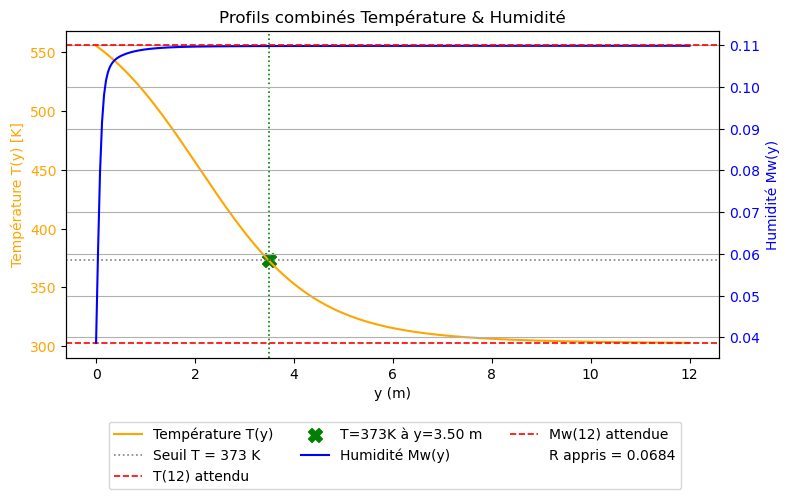
\includegraphics[width=0.7\linewidth]{py6}
	\caption{Graphe combiné de $T(y)$ et de $M_w(y)$ en fonction de $y$ à l'aide des PINNs}.
	\label{fig:py6}
\end{figure}
\begin{figure}[]
	\centering
	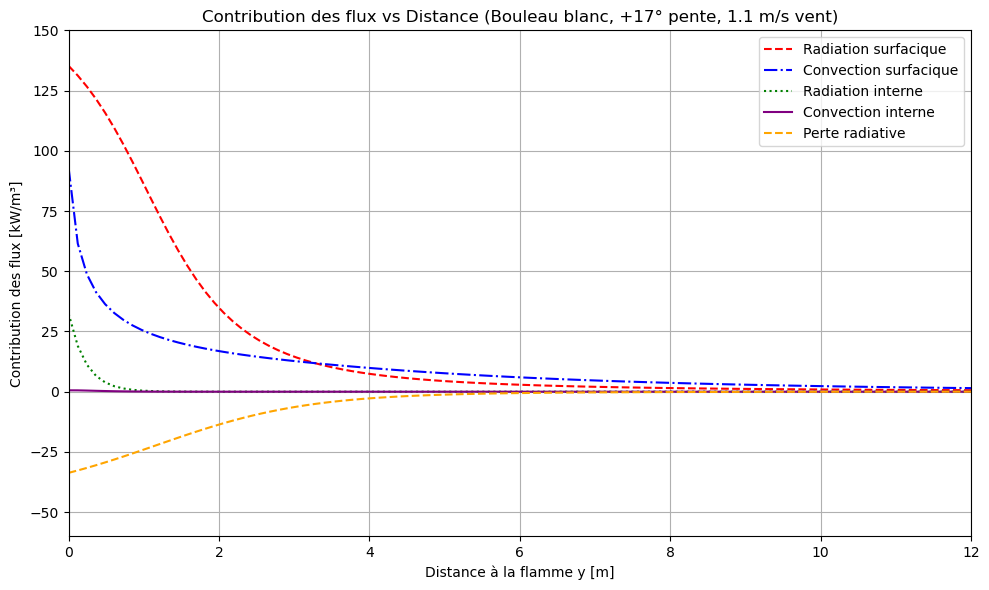
\includegraphics[width=0.7\linewidth]{py5}
	\caption{Contribution de chaque flux en fonction de $y$ à l'aide des PINNs}
	\label{fig:py5}
\end{figure}
\clearpage	

\begin{landscape}
	\begin{table}[]
		\Huge
		\centering
		\caption{Valeurs numériques des différents profils et flux en fonctions de $y$}
		\label{tab:final}
		\begin{tabular}{@{}lrrrrrrrr@{}}
			\toprule
			$y$ (m) & $T$ (K) & $M_w$ & $q_{\text{rs}}$ & $q_{\text{cs}}$ & $q_{\text{ri}}$ & $q_{\text{ci}}$ & $q_{\text{pr}}$ & $Q_1$ ($\mathrm{kW/m^3}$)\\
			\midrule
			0.0  & 556.6 & 0.039& 135.2  & 92.8 & 32.3 & 0.7   & -33.7 & 227.4 \\
			1.0  & 535.8 & 0.106 & 86.0  & 25.2 & 0.4   & 0.1 & -24.0 & 87.7  \\
			2.0  & 456.7 & 0.109 & 34.8  & 16.8  & 0.0   & 0.0   & -13.6 & 38.0  \\
			4.0  & 353.1 & 0.1100 & 7.4   & 9.9  & 0.0   & 0.0   & -2.8 & 14.5  \\
			6.0  & 315.5 & 0.1100 & 2.9   & 6.0  & 0.0   & 0.0   & -0.6 & 8.3 \\
			8.0  & 306.4 & 0.1100 &1.5   & 3.7  & 0.0   & 0.0   & -0.2  & 5.0  \\
			12.0 & 303.0 & 0.1100 & 0.6   &1.5   & 0.0   & 0.0   & -0.0   & 2.1   \\
			\bottomrule
		\end{tabular}
	\end{table}
\end{landscape}
\clearpage
Lorsque la température du combustible dépasse légèrement $373\,\mathrm{K}$, correspondant à la température d’ébullition de l’eau, l’humidité décroît alors fortement, à une vitesse $R = 0{,}068$.  
Cette chute rapide s’explique par la rupture des liaisons des molécules d’eau ($\mathrm{H_2O}$), provoquée par la température atteinte. Le combustible s’assèche ainsi rapidement.  
Une fois que toute l’humidité a été évacuée ($M_w(0) = 0$), son taux reste constant jusqu’à la fin du processus de pyrolyse.

La figure~\ref{fig:py5} montre que la radiation surfacique est le flux dominant. Elle correspond au transfert de chaleur par rayonnement de la flamme vers la surface du combustible. Elle est suivie par la convection surfacique et les pertes radiatives, qui restent significatives comparées aux flux internes. Cela montre que les échanges thermiques à la surface du lit de combustible sont plus importants que ceux à l’intérieur.
\subsection{Discussion}
Les profils de température et d’humidité obtenus sont en accord avec les lois physiques du phénomène. En effet, à mesure que le combustible se rapproche de la flamme, sa température augmente progressivement. Elle tend alors vers la température d’inflammation, fixée à $561,\mathrm{K}$. Parallèlement, l’humidité contenue dans le combustible décroît progressivement. Elle s’annule autour de $373,\mathrm{K}$, température correspondant à l’ébullition de l’eau. La vitesse de propagation est alors estimée constante : $R = 0{,}068$.

Par ailleurs, l’importance de la chaleur à la surface du combustible confirme l’hypothèse selon laquelle la flamme est considérée comme l’unique source de chaleur. Hormis quelques écarts, les flux obtenus concordent très bien avec ceux de \textbf{Koo \textit{et al.} (2005)}. Le décalage observé dans le profil de l’humidité $M_w$ provient d’une mauvaise détection de l’instant de transition. Celle-ci n’est pas bien identifiée par le sous-problème SP2. Plusieurs facteurs peuvent expliquer cette imprécision : les paramètres numériques supposés, la gestion imparfaite de la discontinuité via la fonction douce $\mathcal{X}(y)$, ou encore un déséquilibre dans les coefficients de pénalisation. Ces éléments illustrent l’une des limites des PINNs classiques.

Malgré cela, l’approche proposée a validé plusieurs aspects du modèle. Elle a permis d’imposer précisément les conditions initiales, d’estimer automatiquement la vitesse $R = 0{,}068$, d’identifier le moment de transition, et de restituer les profils de $T$, $M_w$ et des différents flux. Les solutions obtenues, par construction, sont globales, continues et différentiables, conformément aux propriétés des réseaux de neurones utilisés.


	
	\chapter*{Conclusion et Perspective}  
	\addcontentsline{toc}{chapter}{Conclusion et Perspective}
	\vspace{-0.4cm}
	
Dans ce document, nous avons étudié un modèle physique simplifié de propagation du feu dans un lit de combustible poreux, inspiré des travaux de \textbf{Koo \textit{et al.} (2005)}.
Ce modèle a été formulé sous la forme d’un système hybride. Il est composé de deux régimes d’équations différentielles ordinaires (SP1 et SP2). Ces régimes s’activent selon une condition imposée sur la température locale : $T(y) = 373, \mathrm{K}$.
L’analyse mathématique a montré que le modèle constitue un système hybride stable par morceaux. Ce système admet des solutions globales.
Cependant, en raison de sa nature (transitions brutales, discontinuités, non-linéarités, etc.), les méthodes analytiques ou numériques classiques rencontrent des difficultés.
Seule la méthode de Runge-Kutta d’ordre 4 (RK4) a permis d’obtenir des résultats relativement satisfaisants.
Par ailleurs, nous avons implémenté la méthode des réseaux de neurones physiquement informés (PINNs), dans sa version classique.
Cette approche transforme le système initialement discontinu en un système continu. Cette transformation est rendue possible grâce à une fonction d’activation douce centrée autour de $T = 373, \mathrm{K}$.
Elle a permis d’obtenir des solutions globales, continues et différentiables. Ces solutions valident plusieurs aspects dynamiques du modèle, tout en respectant la réalité physique du phénomène.
Comme prévu dans nos objectifs, cette méthode nous a permis d’estimer simultanément les trois variables clés du système : la température $T(y)$, l’humidité $M_w(y)$ et la vitesse de propagation $R$.
Toutefois, les résultats obtenus avec la méthode RK4 restent globalement meilleurs.
En considérant les états comme discontinus, RK4 offre une solution plus directe. Elle demande aussi moins de ressources en temps de calcul que l’apprentissage avec les PINNs.
L’apprentissage profond permet une inférence rapide une fois le modèle entraîné.
Cependant, la phase d’entraînement initiale est plus longue que les méthodes classiques.
Comme le soulignent \textbf{Raissi \textit{et al.} (2019)}, les PINNs ne sont pas conçus pour résoudre des problèmes directs.
Ils ne rivalisent pas avec les méthodes numériques classiques en termes d’efficacité et de précision. Leur véritable avantage réside dans leur capacité à intégrer des données réelles. Cela permet d’ajuster le modèle et d’en améliorer les performances.
En résumé, cette étude confirme que l’on peut appliquer les PINNs à des problèmes physiques. Cela est possible à condition de bien gérer les discontinuités. Il faut aussi pouvoir reformuler ces problèmes en systèmes d’équations différentielles ordinaires avec transitions de régime.

Au regard des difficultés rencontrées pour atteindre la précision des méthodes numériques classiques et reproduire fidèlement les résultats obtenus par \textbf{Koo \textit{et al.} (2005)}, il apparaît essentiel d’envisager les pistes suivantes pour améliorer les performances des PINNs dans ce type de problèmes :

\begin{itemize}
	\item[$\maltese$] \textbf{Combiner les PINNs à la méthode de tir} afin d’imposer avec précision les conditions de référence, notamment aux frontières du domaine.
	
	\item[$\maltese$] \textbf{Utiliser une méthode numérique classique} pour détecter précisément les instants de transition entre les régimes, puis appliquer les PINNs séparément sur chaque sous-système identifié.
	
	\item[$\maltese$] \textbf{Utiliser des variantes améliorées des PINNs}, telles que les {Extended PINNs} (XPINNs), qui consistent à découper le domaine en plusieurs sous-domaines, chacun étant traité par un réseau distinct.  
	Cette approche permet une meilleure gestion des discontinuités et des transitions brutales entre régimes.
\end{itemize}


	
	\clearpage
\chapter*{Références Bibliographiques}
\addcontentsline{toc}{chapter}{Références Bibliographiques}
\begin{flushleft}
	
	Alur R., Courcoubetis C., Henzinger T.A. et Ho P.H., 1993. Hybrid Automata: An Algorithmic Approach to the Specification and Verification of Hybrid Systems. Computers science, 170, 209-229.
	
	\vspace{0.1cm}
	Ascher U.M. et Petzold L.R., 1998. Computer Methods for Ordinary Differential Equations and Differential-Algebraic Equations. 314p. Philadelphia, PA.
	
		\vspace{0.1cm}
	Branicky M. S., 1995. Studies in Hybrid Systems : Modeling, Analysis, and Control, 199p. Massachusetts Institute of Technology.
	
		\vspace{0.1cm}
	Branicky M. S. 1998. Multiple Lyapunov functions and other analysis tools for swit-ched and hybrid systems. IEEE Transactions on Automatic Control, 43, 475-482.
	
		\vspace{0.1cm}
	Branicky M. 2005. Introduction to Hybrid Systems. Department of Electrical Engineering and Computer Science. 114, 91-116.
	
		\vspace{0.1cm}
	Buckmaster J.D., Ludford G.S.S., 1982. Theory of Laminar Flames. 266p. Cambridge University Press
	
		\vspace{0.1cm}
	Chen F., Sondak D., Protopapas P., Mattheakis M., Liu S., Agarwal D. et Di Giovanni M., 2020. NeuroDiffEq : A Python package for solving differential equations with neural networks. Journal of Open Source Software, 5(52), 1931.
	
		\vspace{0.1cm}
	De Curtò J. et De Zarzà I., 2024. Hybrid State Estimation : Integrating Physics-Informed Neural Networks with Adaptive UKF for Dynamic Systems. Electronics, 13(11), 2208.
	
		\vspace{0.1cm}
	Dizet N., Porterie B., Pizzo Y., Mense M., Sardoy N., Alibert D., Louiche J., Porterie T. et Pouschat P., 2022. Analyse des risques d’incendie dans les grandes structures à compartiments multiples à l’aide d’une approche hybride multi-échelle. Sciences appliquées, 12(9), 4123.
	
		\vspace{0.1cm}
	Dupuy J.L. et Pimont F., 2009. Modélisation du feu : une technologie puissante pour la simulation et la prédiction de la propagation. Revue Scientifique et Technique Forêt et Environnement du Bassin du Congo, 185, 18-19.
	
	\clearpage
	
	Filippov A.F., 1988. Differential Equations with Discontinuous Righthand Sides. Kluwer Academic Publishers, 18, 1988.
	
		\vspace{0.1cm}
	Gallouët T., Treust L., Vladuts S., 2022. Équations différentielles ordinaires. 108p. Université d’Aix-Marseille, France.
	
		\vspace{0.1cm}
	Goebel R., Sanfelice R.G. et Teel A.R., 2012. Hybrid Dynamical Systems : Modeling, Stability, and Robustness. 232p. Princeton University Press.
	
		\vspace{0.1cm}
	Hairer E., Norsett S.P. et Wanner G., 1987. Solving Ordinary Differential Equations I. 523p, Springer-Verlag.
	
		\vspace{0.1cm}
	Hedfi A.T., 2013. Surveillance par observateurs des systèmes dynamiques hybrides, 133p. Université de Lille 1.
	
		\vspace{0.1cm}
	Irsalinda N., Bakar M.A., Harun F., Surono S. et Pratama D.A., 2025. A New Hybrid Approach for Solving Partial Differential Equations : Combining Physics-Informed Neural Networks with Cat-and-Mouse Based Optimization. Results in Applied Mathematics, 25, 100-539.
	
		\vspace{0.1cm}
	Kazuyuki A. et Suzuki H., 2010. Theory of hybrid dynamical systems and its applications to biological and mediacal systems, 365, 4893-4914 
	
		\vspace{0.1cm}
	Khalil H.K., 2002. Nonlinear Systems. 3rd, Prentice Hall. 
	
		\vspace{0.1cm}
	Koo E., Pagni P., Woycheese J., Stephens S., Weise D. et Huff J., 2005. A Simple Physical Model for Forest Fire Spread Rate. Fire Safety Science, 8, 851-862.
	
		\vspace{0.1cm}
	Lei C., Matsuzawa H., Peng R. et Zhou M., 2021. Refined estimates for the propagation speed of the transition solution to a free boundary problem with a nonlinearity of combustion type. Journal of Differential Equations, 301, 1-32.
	
		\vspace{0.1cm}
	Liberzon D., 2003. Switching in Systems and Control. 190p, Springer-verlag.
	
		\vspace{0.1cm}
	Lygeros J., Johansson K.H., Simic S.N., Zhang J. et Sastry S.S., 2003. Dynamical properties of hybrid automata. IEEE Transactions on Automatic Control, 48, 2-17.
	
		\vspace{0.1cm}
	Mecence R., 2018. Equations différentielles à retard dépendant de l'état. 43p. Centre universitaire Belhadj Bouchaib d'Ain-Témouchent. 
	
		\vspace{0.1cm}
	Mele A. et Pironti A., 2024. Stabilization of Nonlinear Systems by Neural Lyapunov Approximators and Sontag’s Formula. 2024. IEEE.
	
		\vspace{0.1cm}
	Mullins M., 2025. Réseaux de neurones informés par la physique pour la résolution d’équations de mécanique des fluides. 144p. Université du Quebec, Montréal. 
	
	\clearpage
	
	Pimont F., 2008. Modélisation physique de la propagation des feux de forêts : Effets des caractéristiques physiques du combustible et de son hétérogénéité. 326p. Université d’Aix-Marseille.  
	
		\vspace{0.1cm}
	Pujo M.L., 1918. Équations différentielles ordinaires et partielles. 47p. Université Claude Bernard - Lyon I.
	
		\vspace{0.1cm}
	Raissi M., Perdikaris P., Ahmadi N. et Karniadakis G., 2024. Physics-Informed Neural Networks and Extensions. International Press, 1-8. 
	
		\vspace{0.1cm}
	Raissi M., Perdikaris P. et Karniadakis G. E., 2019. Physics-informed neural networks : A deep learning framework for solving forward and inverse problems involving nonlinear partial differential equations. Journal of Computational Physics, 378, 686-707.
	
		\vspace{0.1cm}
	Schiulaz M., Laumann C.R., Balatsky A.V. et Spivak B.Z., 2018. Theory of combustion in disordered media. Physical Review E, 97(6), 062-133.
	
		\vspace{0.1cm}
	Zhang Z., Wang Q., Zhang Y., Shen T. et Zhang W., 2025. Physics-informed neural networks with hybrid Kolmogorov-Arnold network and augmented Lagrangian function for solving partial differential equations. Scientific Reports, 15(1), 10523.
	
\end{flushleft}

	
	
	
	%%% Références (style Vancouver)
	%	\printbibliography[title=Références Bibliographiques]
	%	\addcontentsline{toc}{chapter}{Références Bibliographiques}
	
	% Annexes
	\appendix
	\chapter*{Annexe I : Expression des constantes physiques}
	\addcontentsline{toc}{chapter}{Annexe I : Expression des constantes physiques}
	\label{chp:annexe I}
	\begin{align*}
		a &= \frac{1}{\cos\theta L_{\text{fl}}}, \quad b=\tan\theta, \quad r=0.25s, \quad c=\frac{0.3}{L_{\text{fl}}} \\ 
		\\
		\gamma_1& = \rho_f C_{\text{pf}} \phi, \quad \gamma_2 = \rho_f h_{\text{vap}} \phi,  \quad \alpha_2 = rE_b\\
		\\
		\alpha_1 &= \frac{a_{fb}E_{fl}}{2l_f}\tanh\left(\frac{2}{3}\left(\frac{w}{L_{fl}}\right)^{1/3}\right) , \quad \alpha_3 = -\frac{\epsilon_{fb}\sigma}{l_f} \\
		\\
		\alpha_4 &= \frac{0.565k_{fl}(\rho u)^{1/2}\mathrm{Pr}^{1/2}}{\mu l_f}, \quad \alpha_5 = \frac{0.565k_\infty(\rho u)^{1/2}}{\mu l_f} \\
		\\
		\alpha_6 &= \frac{0.911sk_b\mathrm{Re}_D^{0.385}\mathrm{Pr}^{1/3}}{D}, \quad \alpha_7 = \frac{0.911sk_\infty\mathrm{Re}_D^{0.385}\mathrm{Pr}^{1/3}}{D}
	\end{align*}
	

	\pagenumbering{roman}
	\chapter*{Annexe II : Illustration du corps}
	\addcontentsline{toc}{chapter}{Annexe II : Illustration du corps}
	\label{chp:annexe II}
	
	\begin{figure}[h]
		\centering
		\includegraphics[width=0.6\linewidth]{im9}
		\caption{De l'intelligence artificielle aux réseaux de neurones PINNs.}
		\label{fig:im9}
	\end{figure}
		\begin{figure}[h]
	\centering
	\includegraphics[width=0.6\linewidth]{im16}
	\caption{Propagation du feu en situation réel dans une végétation dense.}
	\label{fig:im16}
\end{figure}
	\begin{figure}[h]
		\centering
		\includegraphics[width=0.6\linewidth]{im14_1}
		\caption{Schéma du "Event-Driven"}
		\label{fig:im141}
	\end{figure}

\chapter*{Annexe III : Codes sources : Python}
\addcontentsline{toc}{chapter}{Annexe III : codes sources}
\label{chp:annexe III}

\begin{lstlisting}[style=pythonstyle]
import torch, import math, import torch.nn as nn, import numpy as np, import torch.autograd as autograd, import matplotlib.pyplot as plt, import torch, torch.nn as nn, torch.nn.functional as F
# ========== DÉFINITION DES PARAMÈTRES PHYSIQUES ==========
sigma = 5.67e-8, lf = 0.114, L_fl = 1.69, Uw = 1.1, Omega_s_deg = 17, Omega_s = math.radians(Omega_s_deg), rho_f = 609, phi = 0.008, cp_f = 2500, h_vap = 2.25e6, T_ig = 561.0, T_inf = 303.0, Mw_inf=0.11, T_fl = 1083.0, T_b = 561.0, D = 0.00252, w = 0.686, afb = 0.6, eps_fb = 0.9, s = 17.5, k_fl = 0.1, k_b = 0.0495, mu = 6.2e-5, Pr = 0.71
# === Fonctions intermediares  ===
def Omega_w(Uw=Uw, g=9.81, L_fl=L_fl):
Uw_t = torch.tensor(Uw), gL_t = torch.tensor(g * L_fl)
return torch.atan(1.4 * Uw_t / torch.sqrt(gL_t))
def theta(Uw=Uw, Omega_s=Omega_s):
return torch.tensor(Omega_s) + Omega_w(Uw)
def Z(y, L_fl=L_fl):
th = theta()
return (y / L_fl - torch.sin(th)) / torch.cos(th)
# === definition des flux ===
def epsilon_fl(L_fl=L_fl):
return 1 - torch.exp(torch.tensor(-0.6 * L_fl))
def E_fl():  # Flux émis par la flamme
return epsilon_fl() * sigma * T_fl**4
def E_b():
return sigma * T_b**4
def q_rs(y):  # Chaleur par rayonnement de la flamme
Z_val = Z(y), tanh_term = torch.tanh(torch.tensor((2 / 3) * (w / L_fl)**(1 / 3)))
return (afb * E_fl() / (2 * lf)) * (1 - Z_val / torch.sqrt(1 + Z_val**2)) * tanh_term
def q_ri(y):  # Rayonnement du lit de braises
return 0.25 * s * E_b() * torch.exp(-0.25 * s * y)
def q_pr(y, T):  # Rayonnement des braises
return -eps_fb * sigma / lf * (T**4 - T_inf**4) #expression non linearisé
def Re_y(y):  # Nombre de Reynolds local
return rho_f * Uw * y / mu
def q_cs(y, T):
eps = 1e-1, y_safe = y + eps, Re = Re_y(y_safe), coeff = 0.565 * k_fl * Re.sqrt() * Pr**0.5, base = y_safe * lf, exponent = torch.exp(-0.3 * y_safe / L_fl), q_val = coeff / base * (T_fl - T) * exponent
return q_val 
def Re_D():
U_fb = (1 - phi) * Uw
return rho_f * U_fb * D / mu
def q_ci(y, T):  # Convection du lit de braises
Re = Re_D()
return (0.911 * s * k_b * Re**0.385 * Pr**(1 / 3)) / D * (T_b - T) * torch.exp(-0.25 * s * y)
def Q_1(y, T):
q = q_rs(y) + q_ri(y) + q_pr(y, T) + q_cs(y, T) + q_ci(y, T)
return q
def Q_2(y):
"""Calcule de Q_2(y) à T=373K"""
T_fixed = torch.tensor(373.0).to(y.device), q_rs_val = q_rs(y), q_ri_val = q_ri(y), q_pr_val = q_pr(y, T_fixed), q_cs_val = q_cs(y, T_fixed), q_ci_val = q_ci(y, T_fixed)
return q_rs_val + q_ri_val + q_pr_val + q_cs_val + q_ci_val
# -----Réseau de base----------
class Net(nn.Module):
def __init__(self, out_scale=1.0):
super().__init__()
self.net = nn.Sequential(
nn.Linear(1, 64), nn.Tanh(),
nn.Linear(64, 64), nn.Tanh(),
nn.Linear(64, 1)
)
self.out_scale = out_scale
def forward(self, y):
return self.out_scale * torch.sigmoid(self.net(y))
# ------Modèle : T(y), Mw(y) et paramètre R appris--------------
class JointModel(nn.Module):
def __init__(self, lambda_chi=1000.0, R_min=0.0, R_max=0.08):
super().__init__()
self.T_net  = Net(out_scale=300.0)
self.Mw_net = Net(out_scale=0.11)
self.R_raw  = nn.Parameter(torch.tensor(0.0))
self.lambda_chi = lambda_chi
self.R_min = R_min
self.R_max = R_max
def forward(self, y):
T  = 300.0 + self.T_net(y)
Mw = self.Mw_net(y)
return T, Mw
def R(self):
return self.R_min + (self.R_max - self.R_min) * torch.sigmoid(self.R_raw)
def chi(self, T):
return torch.sigmoid(self.lambda_chi * (T - 373.0))
# ----------------Boucle dentrainement------------------------------------------
def train_joint_model(n_epochs=10000, lambda_chi=10000.0, lr=1e-3):
model     = JointModel(lambda_chi=lambda_chi).to(device)
optimizer = torch.optim.Adam(model.parameters(), lr=lr)
# points de collocation
y_train = torch.linspace(0, 12, 120, device=device).view(-1, 1)
y_train.requires_grad_()
for epoch in range(n_epochs):
optimizer.zero_grad()
T, Mw = model(y_train)
R     = model.R()
chi   = model.chi(T)
# dérivées
dT_dy  = autograd.grad(T,  y_train, torch.ones_like(T),  create_graph=True)[0]
dMw_dy = autograd.grad(Mw, y_train, torch.ones_like(Mw), create_graph=True)[0]
# résidus pondérés
res_T  = (1 - chi) * (dT_dy + Q_1(y_train, T) / (rho_f * cp_f  * phi * R))
res_Mw = chi       * (dMw_dy - Q_2(y_train)   / (rho_f * h_vap * phi * R))
loss_pde = torch.mean(res_T**2 + res_Mw**2)
# condition initiale en y = 12  (T= T_inf, Mw = Mw_inf)
y_ic = torch.tensor([[12.0]], device=device)
T_ic, Mw_ic = model(y_ic)
loss_ic = (9_0000 * (T_ic - T_inf)**2 + 1e20 * (Mw_ic - Mw_inf)**2)
loss = loss_pde + loss_ic
loss.backward()
optimizer.step()
if epoch % 500 == 0:
print(f"Epoch {epoch:5d} | loss={loss.item():.3e} | R={R.item():.4f}")
return model
# -----------------Entraînement--------------------------------
model = train_joint_model(n_epochs=5000, lambda_chi=100)
with torch.no_grad():
R_learned = model.R().item()
print(f"\nParamètre R appris : {R_appris:.4f}")
# ------------------profils fins------------------------------------
y_fine = torch.linspace(0, 12, 600, device=device).view(-1, 1)
T_val, Mw_val = model(y_fine)
y_np  = y_fine.cpu().numpy().flatten()
T_np  = T_val.cpu().numpy().flatten()
Mw_np = Mw_val.cpu().numpy().flatten()
# === Analyse post-entraînement pour extraire les valeurs ===
with torch.no_grad():
y_fine = torch.linspace(0, 12, 1000, device=device).view(-1, 1)
T_vals, Mw_vals = model(y_fine)
target_temp = 373.0
diffs = torch.abs(T_vals - target_temp)
min_diff, idx = torch.min(diffs, dim=0)
y_target = y_fine[idx].item()
target_Mw = 0.11
diffs_Mw = torch.abs(Mw_vals - target_Mw)
min_diff_Mw, idx_Mw = torch.min(diffs_Mw, dim=0)
y_Mw_target = y_fine[idx_Mw].item()
T0 = model(torch.tensor([[0.0]], device=device))[0].item()
T12 = model(torch.tensor([[12.0]], device=device))[0].item()
Mw0 = model(torch.tensor([[0.0]], device=device))[1].item()
Mw12 = model(torch.tensor([[12.0]], device=device))[1].item()
# === Tracé des résultats avec y_target ===
def plot_results(model, y_target, y_Mw_target):
y = torch.linspace(0, 12, 300, device=device).view(-1, 1), T, Mw = model(y), y_np = y.cpu().detach().numpy(), T_np = T.cpu().detach().numpy(), Mw_np = Mw.cpu().detach().numpy()
plt.figure(figsize=(10, 4))
# === Température ===
plt.subplot(1, 2, 1)
plt.plot(y_np, T_np, label="Température T(y)", color='orange')
plt.axhline(T_inf, color='red', linestyle='--', label="T(12) attendu")
plt.axhline(373, color='gray', linestyle=':', linewidth=1.2, label="Seuil T = 373 K")
plt.scatter([y_target], [373], color='green', marker='X', s=100, label=f"T=373K à y={y_target:.2f} m")
plt.axvline(x=y_target, color='green', linestyle=':', linewidth=1.2)
plt.xlabel("y (m)"); plt.ylabel("T (K)")
plt.title("Profil de Température"); plt.grid(); plt.legend()
# === Humidité ===
plt.subplot(1, 2, 2)
plt.plot(y_np, Mw_np, label="Humidité Mw(y)", color='blue')
plt.axhline(Mw_inf, color='red', linestyle='--', label="Mw(12) attendue")
plt.scatter([y_Mw_target], [0.11], color='purple', marker='X', s=100, label=f"Mw=0.11 à y={y_Mw_target:.2f} m")
plt.axvline(x=y_Mw_target, color='purple', linestyle=':', linewidth=1.2)
plt.xlabel("y (m)"); plt.ylabel("Mw")
plt.title("Profil d’Humidité"); plt.grid(); plt.legend()
plt.tight_layout()
plt.show()
plot_results(model, y_target, y_Mw_target)
#==================graphe combinée==========
def plot_combined_graph(model, y_target):
y = torch.linspace(0, 12, 300, device=device).view(-1, 1)
T, Mw = model(y)
y = y.cpu().detach().numpy().flatten()
T = T.cpu().detach().numpy().flatten()
Mw = Mw.cpu().detach().numpy().flatten()
fig, ax1 = plt.subplots(figsize=(8, 4))
# ------------------------------------------Axe 1 : Température--------------
ax1.set_xlabel("y (m)")
ax1.set_ylabel("Température T(y) [K]", color='orange')
ax1.plot(y, T, color='orange', label="Température T(y)")
ax1.axhline(373, color='gray', linestyle=':', linewidth=1.2, label="Seuil T = 373 K")
ax1.axhline(T_inf, color='red', linestyle='--', label="T(12) attendu")
ax1.axvline(x=y_target, color='green', linestyle=':', linewidth=1.2)
ax1.scatter([y_target], [373], color='green', marker='X', s=100, label=f"T=373K à y={y_target:.2f} m")
ax1.tick_params(axis='y', labelcolor='orange')
# ---------------------------------Axe 2 : Mw------------------------------
ax2 = ax1.twinx()
ax2.set_ylabel("Humidité Mw(y)", color='blue')
ax2.plot(y, Mw, color='blue', label="Humidité Mw(y)")
ax2.axhline(Mw_inf, color='red', linestyle='--', label="Mw(12) attendue")
ax2.tick_params(axis='y', labelcolor='blue')
#------------------------------- Légende combinée-------------------------------
lines1, labels1 = ax1.get_legend_handles_labels()
lines2, labels2 = ax2.get_legend_handles_labels()
fig.legend(lines1 + lines2, labels1 + labels2, loc='lower center', bbox_to_anchor=(0.5, -0.2), ncol=2)
fig.tight_layout()
plt.title("Profils combinés Température & Humidité")
plt.grid()
plt.show()
plot_combined_graph(model, y_target)
# === Résumé imprimé ===
print("\n=== Résumé des résultats ===")
#print(f"Valeur de R utilisée : {R}")
print(f"y* tel que T(y*) ≈ 373 K : y = {y_target:.4f} m")
print(f"y* tel que Mw(y*) ≈ 0.11 : y = {y_Mw_target:.4f} m")
print(f"T(0)  = {T0:.2f} K")
print(f"T(12) = {T12:.2f} K")
print(f"Mw(0)  = {Mw0:.5f}")
print(f"Mw(12) = {Mw12:.5f}")
# ==== Paramètres ====
l_f = 0.114 
y = torch.linspace(0, 12, 100).view(-1, 1).to(device)
# Récupération des profils T et Mw
with torch.no_grad():
T_pred, Mw_pred = model(y), T = T_pred.detach(), Mw = Mw_pred.detach()
# Calcul des flux volumiques (en kW/m³)
q_rs_vol = q_rs(y).detach().cpu().numpy().flatten() / l_f 
q_ri_vol = q_ri(y).detach().cpu().numpy().flatten() / l_f 
q_cs_vol = q_cs(y, T).detach().cpu().numpy().flatten() / l_f 
q_pr_vol = q_pr(y, T).detach().cpu().numpy().flatten() / l_f 
q_ci_vol = q_ci(y, T).detach().cpu().numpy().flatten() / l_f 
# ==== Tracé des contributions ====
plt.figure(figsize=(10, 6))
plt.plot(y.cpu().numpy(), q_rs_vol, label='Radiation surfacique', linestyle='--', color='red')
plt.plot(y.cpu().numpy(), q_cs_vol, label='Convection surfacique', linestyle='-.', color='blue')
plt.plot(y.cpu().numpy(), q_ri_vol, label='Radiation interne', linestyle=':', color='green')
plt.plot(y.cpu().numpy(), q_ci_vol, label='Convection interne', color='purple')
plt.plot(y.cpu().numpy(), q_pr_vol, label='Perte radiative', linestyle='--', color='orange')
plt.xlabel('Distance à la flamme y [m]')
plt.ylabel('Contribution des flux [kW/m³]')
plt.title('Contribution des flux vs Distance (Bouleau blanc, +17° pente, 1.1 m/s vent)')
plt.legend()
plt.grid(True)
plt.xlim(0, 12)
plt.ylim(-60, 150)
plt.tight_layout()
plt.show()
y_values = torch.tensor([[0.0, 1.0, 2.0, 4.0, 6.0, 8.0, 12.0]], device=device).T
T_values, Mw_values = model(y_values)
print("  y (m) | T(y) (K) | Mw(y) |  q_rs  |  q_cs  |  q_ri  |  q_ci  |  q_pr   | Total")
print("----------------------------------------------------------------------------")
for y_i, T_i, Mw_i in zip(y_values, T_values, Mw_values):
q_rs_val = q_rs(y_i).item() / l_f 
q_cs_val = q_cs(y_i, T_i).item() / l_f 
q_ri_val = q_ri(y_i).item() / l_f 
q_ci_val = q_ci(y_i, T_i).item() / l_f 
q_pr_val = q_pr(y_i, T_i).item() / l_f 
total = q_rs_val + q_cs_val + q_ri_val + q_ci_val + q_pr_val
print(f"{y_i.item():6.1f} | {T_i.item():7.1f} | {Mw_i.item():5.3f} | {q_rs_val:6.1f} | {q_cs_val:6.1f} | {q_ri_val:6.1f} | {q_ci_val:6.1f} | {q_pr_val:7.1f} | {total:6.1f}")
\end{lstlisting}




\end{document}